\documentclass[runningheads]{llncs}

\usepackage{amsmath,amssymb,mathtools}
\usepackage{graphicx,booktabs}
\usepackage[expansion=false]{microtype}
\usepackage[hidelinks]{hyperref}
\spnewtheorem{assumption}[theorem]{Assumption}{\bfseries}{\itshape}
\newcommand{\R}{\mathbb R}
\newcommand{\E}{\mathbb E}
\newcommand{\Prob}{\mathbb P}
\newcommand{\KL}{D_{\mathrm{KL}}}
\newcommand{\logit}{\operatorname{logit}}
\newcommand{\sigmoid}{\operatorname{expit}}
\newcommand{\BF}{\mathrm{BF}}
\newcommand{\IG}{\mathrm{IG}}
% Automatically generated numerical values.
\newcommand{\SimulationHistories}{2000}
\newcommand{\SymmetryMaxLogBF}{0.0}
\newcommand{\StabilityViolations}{0}
\newcommand{\StabilityMaxRatio}{0.0094}
\newcommand{\FixedMarginalBrier}{0.149}
\newcommand{\FixedMarginalLogLoss}{0.454}
\newcommand{\FixedMarginalIG}{0.220}
\newcommand{\FixedMarginalAccuracy}{0.782}
\newcommand{\FixedOracleBrier}{0.137}
\newcommand{\FixedOracleLogLoss}{0.420}
\newcommand{\FixedOracleIG}{0.268}
\newcommand{\FixedOracleAccuracy}{0.794}
\newcommand{\FixedLastBrier}{0.363}
\newcommand{\FixedLastLogLoss}{1.878}
\newcommand{\FixedLastIG}{0.498}
\newcommand{\FixedLastAccuracy}{0.582}
\newcommand{\PriorMarginalBrier}{0.133}
\newcommand{\PriorMarginalLogLoss}{0.409}
\newcommand{\PriorMarginalIG}{0.280}
\newcommand{\PriorMarginalAccuracy}{0.807}
\newcommand{\PriorOracleBrier}{0.112}
\newcommand{\PriorOracleLogLoss}{0.344}
\newcommand{\PriorOracleIG}{0.337}
\newcommand{\PriorOracleAccuracy}{0.836}
\newcommand{\PriorLastBrier}{0.384}
\newcommand{\PriorLastLogLoss}{2.502}
\newcommand{\PriorLastIG}{0.526}
\newcommand{\PriorLastAccuracy}{0.568}
\newcommand{\DependentMarginalBrier}{0.171}
\newcommand{\DependentMarginalLogLoss}{0.529}
\newcommand{\DependentMarginalIG}{0.313}
\newcommand{\DependentMarginalAccuracy}{0.747}
\newcommand{\DependentOracleBrier}{0.151}
\newcommand{\DependentOracleLogLoss}{0.473}
\newcommand{\DependentOracleIG}{0.356}
\newcommand{\DependentOracleAccuracy}{0.783}
\newcommand{\DependentLastBrier}{0.406}
\newcommand{\DependentLastLogLoss}{4.285}
\newcommand{\DependentLastIG}{0.587}
\newcommand{\DependentLastAccuracy}{0.564}

% Generated by code/prepare_paper.py
\newcommand{\EndpointBrierDifference}{-0.112}
\newcommand{\EndpointBrierLower}{-0.121}
\newcommand{\EndpointBrierUpper}{-0.102}
\newcommand{\EndpointLogLossDifference}{-0.274}
\newcommand{\EndpointLogLossLower}{-0.297}
\newcommand{\EndpointLogLossUpper}{-0.251}

\setlength{\emergencystretch}{3em}
\raggedbottom
\begin{document}
\title{When Does Price History Add Information? Endpoint Sufficiency in Prediction Markets}
\titlerunning{Endpoint Sufficiency in Prediction Markets}
\author{Anonymous submission}
\authorrunning{Anonymous}
\institute{}
\maketitle
\begin{abstract}
A prediction-market price is a free forecast, so any method that uses the market's history must beat it. We ask when the history can add outcome information beyond the latest observed price, with the initial price and volume design fixed. The answer depends on which nuisance quantities are unknown. With Gaussian increments of known covariance, an unknown nonnegative response amplitude preserves a directional sufficiency criterion, and information formulas give the proper-score gain when it fails. An unknown common noise scale breaks sufficiency even when the response aligns with the endpoint: the rest of the path then tells how reliable the price signal is, which changes probabilities while preserving the equal-prior decision. For finite mixtures of trading regimes with common outcome tails, the endpoint is never sufficient unless the outcome laws coincide, yet the resulting gain can be negligibly small. A Brier and log-loss decomposition separates this intrinsic value from the approximation and estimation errors of fitted forecasts. In a frozen retrospective study of 2,650 Kalshi BTC and ETH 15-minute contracts, adding a fitted mixture signal to a matched price calibration changes held-out Brier loss by $-0.00011$ (95\% interval $[-0.00053,+0.00028]$) five minutes before close. A matched test of the confidence mechanism, pre-specified and shown by simulation to detect gains of practical size, was then run on a later, untouched cohort of 2,370 contracts. The gain from residual variation had the predicted sign but was practically equivalent to zero: $+0.00008$ in Brier loss (95\% interval $[-0.000001,+0.00016]$). Model-based information and achieved forecasting gains are different quantities, and in this market the price was hard to beat.
\keywords{Prediction markets \and Price discovery \and Sufficiency \and Proper scoring rules \and Market microstructure}
\end{abstract}

\section{Introduction}
A binary prediction-market contract pays one unit if an event occurs and zero otherwise. Its price is a forecast that anyone can read for free, which makes it a demanding baseline for any method that uses the same market's history. Prices track event frequencies well on average \cite{wolfers2004prediction}, although reading them as probabilities depends on beliefs, preferences and trading constraints \cite{manski2006interpreting,wolfers2006interpreting}. Forecasters, oracle designers and market designers all face the same question: when does the history carry outcome information that the price discards?

Throughout, the \emph{endpoint} is the last observed price at the forecast cutoff, before resolution, and not the settlement value. With the initial price fixed, the endpoint is an invertible function of the sum of log-odds increments. We call it \emph{sufficient} when the marginal likelihood ratio depends on the increments only through that sum. Whether it does depends on what the observation model leaves unknown. We therefore study three model classes, each with shared nuisance parameters integrated out, and then test achieved forecasting gains on observed data.

\medskip\noindent\textbf{Contributions.}
\begin{enumerate}
\item With known Gaussian covariance, an unknown nonnegative response amplitude preserves a directional criterion for endpoint sufficiency, and scalar information formulas give the exact proper-score gain when it fails (Sect.~\ref{sec:gauss}).
\item An unknown common noise scale destroys sufficiency even when the mean response aligns with the endpoint. Residual path variation then calibrates confidence in the endpoint signal without changing the equal-prior decision (Sect.~\ref{sec:scale}, Fig.~\ref{fig:scale}).
\item For finite mixtures of trading regimes with a shared nuisance state, common outcome tails imply that the endpoint is sufficient only if the outcome laws coincide. A contamination sweep shows that this strict insufficiency can carry a negligible gain (Sect.~\ref{sec:mixture}).
\item A decomposition of Brier and log risk splits the achieved gain of a fitted history forecast into intrinsic information and two excess-risk terms, which combine approximation and estimation error (Prop.~\ref{prop:decomposition}). It explains how a model can require history dependence while a fitted model loses to the price.
\item A frozen retrospective evaluation on 2,650 Kalshi contracts finds no clear incremental value from fitted history signals over matched price controls (Sect.~\ref{sec:empirical}).
\item A matched test of the confidence mechanism, frozen before evaluation and checked by simulation for sensitivity and for false gains under efficient prices, finds an effect with the predicted sign but practically equivalent to zero on a later cohort of 2,370 contracts (Sect.~\ref{sec:confidence}).
\end{enumerate}
The theory characterizes information under specified observation laws. The experiment tests whether fitted forecasts realize it. We keep the two apart throughout.

\medskip\noindent\textbf{Related work.}
Closest to our question, Richard and Ve\v{c}e\v{r} \cite{richard2021efficiency} test the martingale property of in-play betting quotes, relate likelihood ratios and Bayes factors to trading profits, and find that history-based signals found in training mostly fail out of sample. They test whether past quotes help. We characterize when a prescribed endpoint is sufficient under nuisance-integrated observation laws, and explain why a fitted model can fail even where the model says history matters. Structural models explain how private information moves prices and order flow \cite{kyle1985continuous,glosten1985bid}. Our model derives no equilibrium. It specifies the conditional law of aggregate increments, so its parameters need external estimation or a stated prior. Bayesian inverse problems treat uncertain observation laws and posterior continuity \cite{stuart2010inverse,latz2020wellposedness}, and Bayes factors compare outcome-indexed families \cite{kass1995bayes,chatterjee2020bayes}. Volume-dependent mixing follows the mixture-of-experts construction \cite{jacobs1991adaptive}. Recent empirical work studies calibration across contracts, horizons and platforms \cite{le2026calibration}. We instead compare history models with explicit endpoint recalibrators under proper scoring rules \cite{gneiting2007strictly}. The links between sufficiency and proper scores are classical \cite{pitman1936sufficient,broecker2009reliability}. Our contribution is the dependence of endpoint sufficiency on the nuisance specification (unknown amplitude against unknown scale), the common-tail obstruction for mixtures, and the separation of intrinsic from achieved gains.

\section{Setting and the ideal-price benchmark}
\label{sec:model}
Let $Y\in\{0,1\}$ be the event outcome with prior $\Prob(Y=1)=\pi_0$, where $0<\pi_0<1$ throughout. Fix an initial price $p_0\in(0,1)$ and a volume sequence $v_{1:T}\in[0,\infty)^T$. Observed prices $p_{1:T}$ define log-odds $x_t=\logit(p_t)$ and increments $z_t=x_t-x_{t-1}$. The analysis conditions on $p_0$ and the design. Conditioning on volume defines a conditional experiment and does not remove endogeneity: in $p(Y,\theta\mid z,v)\propto p(z\mid Y,\theta,v)\,p(Y,\theta\mid v)$, volume that depends on the outcome, private information or latent conditions affects both factors, so the prior must condition on it too. We do not derive this likelihood from strategic trading, and our claims are statistical. The simulations draw volumes independently of both. For live forecasting, a sequential factorization with a volume model would replace conditioning on a whole future design.

\paragraph{Information sets.}
The theory compares two forecasts that share $p_0$ and the design:
\[
 r^*=\Prob(Y=1\mid p_0,p_T,v_{1:T}),\qquad q^*=\Prob(Y=1\mid p_0,p_{1:T},v_{1:T}).
\]
Their difference is the value of the intermediate prices once the endpoint, the initial price and the volumes are known. The empirical forecasts of Sect.~\ref{sec:empirical} use other information sets (Table~\ref{tab:infosets}). Those comparisons are practical forecasting tests and do not estimate the theoretical quantity.

\paragraph{Ideal prices.}
Let $\mathcal F_t$ hold the public information at time $t$. If $p_t=\E[Y\mid\mathcal F_t]$, then $(p_t)$ is a bounded martingale and no forecast built from public history improves on $p_t$ in population Brier or log risk \cite{gelman2020information}. Outcome-dependent price changes remain compatible with this benchmark. For $s<t$ and $0<p_s<1$,
\begin{equation}
 \E[p_t-p_s\mid Y=1,\mathcal F_s]=\frac{\operatorname{Var}(p_t\mid\mathcal F_s)}{p_s},\qquad
 \E[p_t-p_s\mid Y=0,\mathcal F_s]=-\frac{\operatorname{Var}(p_t\mid\mathcal F_s)}{1-p_s}.
 \label{eq:outcome-drift}
\end{equation}
The first identity follows from $\E[Yp_t\mid\mathcal F_s]=\E[p_t^2\mid\mathcal F_s]$ by iterated conditioning. The second is analogous. A Gaussian example makes the point concrete. Let $Z_t\mid Y\sim N((2Y-1)\sigma_t^2/2,\sigma_t^2)$ independently, $\Prob(Y=1)=p_0$, and $p_t=\sigmoid(\logit p_0+\sum_{j\leq t}Z_j)$. Each log likelihood ratio equals $Z_t$, so $p_t$ is the posterior probability and a martingale, even though its increments depend on $Y$. An observation law with outcome-dependent drift therefore says nothing against efficient pricing, and a fitted history model that fails to beat the price does not establish efficiency either.

\section{When is the endpoint sufficient?}
\label{sec:endpoint}
The endpoint is an invertible function of $S_T=\sum_tZ_t$ once $p_0$ is fixed. We call it \emph{outcome-sufficient} if $Y$ is conditionally independent of the full increment vector given $(S_T,v)$. Equivalently, the marginal likelihood ratio is a function of $S_T$ alone.

\begin{proposition}[Value of history beyond the endpoint]
\label{prop:history-value}
Under the prior-predictive conditional model, let $q=\Prob(Y=1\mid Z_{1:T},v)$ and $r=\Prob(Y=1\mid S_T,v)$. For logarithmic loss $\mathcal L_{\log}$ and Brier loss $\mathcal L_B$,
\begin{align*}
 \E[\mathcal L_{\log}(r,Y)-\mathcal L_{\log}(q,Y)\mid v]&= I(Y;Z_{1:T}\mid S_T,v),\\
 \E[\mathcal L_B(r,Y)-\mathcal L_B(q,Y)\mid v]&=\E[(q-r)^2\mid v].
\end{align*}
\end{proposition}
\begin{proof}
Expected log loss at a conditional probability is conditional entropy, and $S_T$ is a function of the history. Subtracting the two entropies gives the first identity. For Brier loss, expand $(Y-r)^2$ about $q$ and use $\E[Y-q\mid Z_{1:T},v]=0$.
\end{proof}
The comparison uses the optimal endpoint forecast under the same model. Fitted forecasts add approximation and estimation error on both sides, which the next result makes explicit. It follows from the orthogonality of conditional expectations, as in the sufficiency decompositions of proper scores \cite{broecker2009reliability}.

\begin{proposition}[Intrinsic and achieved gains]
\label{prop:decomposition}
Let $\mathcal E\subseteq\mathcal H$ be the endpoint and history information, $q^*=\Prob(Y=1\mid\mathcal H)$ and $r^*=\Prob(Y=1\mid\mathcal E)$. For any fixed $\mathcal H$-measurable forecast $\widehat q$ and $\mathcal E$-measurable forecast $\widehat r$ with values in $(0,1)$, the Brier identity holds. The log identity holds when both log risks are finite, for example when both forecasts lie in $[\epsilon,1-\epsilon]$ for some $\epsilon>0$:
\begin{align*}
 R_B(\widehat r)-R_B(\widehat q)&=\E(q^*-r^*)^2+\E(\widehat r-r^*)^2-\E(\widehat q-q^*)^2,\\
 R_{\log}(\widehat r)-R_{\log}(\widehat q)&=I(Y;\mathcal H\mid\mathcal E)+\E\,\KL(r^*\|\widehat r)-\E\,\KL(q^*\|\widehat q),
\end{align*}
where $R$ denotes expected loss and $\KL(a\|b)$ is the divergence between Bernoulli laws. For fitted forecasts, the expectations are under the evaluation law with the fitted models held fixed, that is, conditional on the training data.
\end{proposition}
\begin{proof}
For $\mathcal H$-measurable $f$, $\E(Y-f)^2=\E(Y-q^*)^2+\E(q^*-f)^2$. If $f$ is also $\mathcal E$-measurable, $\E(q^*-f)^2=\E(q^*-r^*)^2+\E(r^*-f)^2$ because $\E[q^*\mid\mathcal E]=r^*$. Subtract the two cases. For log loss, $R_{\log}(f)=\E\,h(q^*)+\E\,\KL(q^*\|f)$ with $h$ the binary entropy. For $\mathcal E$-measurable $f$ the terms $\log(r^*/f)$ and $\log\{(1-r^*)/(1-f)\}$ are $\mathcal E$-measurable, so $\E\,\KL(q^*\|f)=\E\,\KL(q^*\|r^*)+\E\,\KL(r^*\|f)$, and $\E\,\KL(q^*\|r^*)=I(Y;\mathcal H\mid\mathcal E)$.
\end{proof}
The first term on each right-hand side is what the theorems below describe. We call the other two excess-risk terms. They include model misspecification and approximation limits of the model class as well as finite-sample error, so more training data need not remove them. A history model can therefore have positive intrinsic value and still lose to a fitted price forecast if its own error is larger. A gain over the raw last price cannot measure $I(Y;Z_{1:T}\mid S_T,v)$.

\begin{table}[t]
\caption{Endpoint sufficiency for the same prescribed endpoint in three model classes, with fixed initial price and design. Each statement uses the assumptions of its proposition. The rows do not form a joint unknown-amplitude and unknown-covariance theorem.}
\label{tab:models}
\centering\small
\begin{tabular}{@{}p{0.27\linewidth}p{0.24\linewidth}p{0.38\linewidth}@{}}
\toprule
Observation model & Nuisance integrated & Endpoint sufficient iff \\
\midrule
Gaussian, known covariance & Response amplitude $A\geq0$ & Response aligns with the covariance-weighted sum direction (Prop.~\ref{prop:ext-sufficiency}) \\[3pt]
Gaussian, known response & Gamma precision & $T=1$ or zero response (Prop.~\ref{prop:scale-sufficiency}) \\[3pt]
Finite mixture, common tail ratios & Finite catalogue state & Marginal outcome laws coincide, $T\geq2$ (Prop.~\ref{prop:mixture-endpoint-tail}) \\
\bottomrule
\end{tabular}
\end{table}

\subsection{Known covariance and an unknown response amplitude}
\label{sec:gauss}
Fix $p_0$, $v_{1:T}$, a known response vector $\boldsymbol a\in\R^T$ and a known positive-definite covariance $\Sigma$, either of which may depend on the design. Let
\begin{equation}
 Z=s_Y A\boldsymbol a+\varepsilon,\qquad \varepsilon\sim N(0,\Sigma),\qquad A\sim\nu,
 \label{eq:ext-model}
\end{equation}
where $s_Y=2Y-1$, $Y$, $A$ and $\varepsilon$ are independent, $A\geq0$, $\Prob(A>0)>0$ and $\E A^2<\infty$. The amplitude $A$ is integrated out. Write $\boldsymbol1$ for the ones vector and set
\begin{align}
 S&=\boldsymbol1^{\mathsf T}Z, & U&=\boldsymbol a^{\mathsf T}\Sigma^{-1}Z, & C&=\boldsymbol1^{\mathsf T}\Sigma\boldsymbol1, & M&=\boldsymbol1^{\mathsf T}\boldsymbol a,\nonumber\\
 J_{\rm H}&=\boldsymbol a^{\mathsf T}\Sigma^{-1}\boldsymbol a, & J_{\rm E}&=M^2/C, & \Delta&=J_{\rm H}-J_{\rm E}. &&
 \label{eq:ext-strengths}
\end{align}
For $j>0$ let $G_j(u)=\int_0^\infty\exp\{\alpha u-\alpha^2j/2\}\nu(d\alpha)$, and $G_0(0)=1$.

\begin{proposition}[Endpoint sufficiency with an unknown amplitude]
\label{prop:ext-sufficiency}
Under \eqref{eq:ext-model}, $\Delta\geq0$. The full-history and endpoint posterior probabilities are
\begin{align}
 q_{\rm H}&=\frac{\pi_0G_{J_{\rm H}}(U)}{\pi_0G_{J_{\rm H}}(U)+(1-\pi_0)G_{J_{\rm H}}(-U)},\nonumber\\
 q_{\rm E}&=\frac{\pi_0G_{J_{\rm E}}(MS/C)}{\pi_0G_{J_{\rm E}}(MS/C)+(1-\pi_0)G_{J_{\rm E}}(-MS/C)}.
 \label{eq:ext-posteriors}
\end{align}
The endpoint is sufficient for $Y$ if and only if
\begin{equation}
 \Delta=0\quad\Longleftrightarrow\quad\boldsymbol a=(M/C)\Sigma\boldsymbol1.
 \label{eq:ext-criterion}
\end{equation}
If $\Delta>0$, the full-history posterior has strictly smaller expected log loss and strictly smaller expected Brier loss than $q_{\rm E}$.
\end{proposition}
The proof is in Appendix~\ref{app:gaussian-extension}. The score gain has an exact scalar form. Let $X=s_YA$ and $W_\gamma=\sqrt\gamma X+N$ with $N\sim N(0,1)$ independent of $(Y,A)$. Write $q_\gamma(w)=\Prob(Y=1\mid W_\gamma=w)$, $I_\nu(\gamma)=I(Y;W_\gamma)$ and $B_\nu(\gamma)=\E[q_\gamma(W_\gamma)\{1-q_\gamma(W_\gamma)\}]$. If $\boldsymbol a\neq0$, then $J_{\rm H}>0$, $U/\sqrt{J_{\rm H}}$ has the scalar law at $\gamma=J_{\rm H}$, and the endpoint has it at $\gamma=J_{\rm E}$ (with $W_0$ uninformative when $M=0$). If $\boldsymbol a=0$, neither carries information. The expected improvements are
\begin{equation}
 G_{\log}=I_\nu(J_{\rm H})-I_\nu(J_{\rm E}),\qquad G_B=B_\nu(J_{\rm E})-B_\nu(J_{\rm H}),
 \label{eq:ext-score-gains}
\end{equation}
and the Gaussian information--MMSE identity \cite{guo2005mutual} gives
\begin{equation}
 G_{\log}=\frac12\int_{J_{\rm E}}^{J_{\rm H}}\E\!\left[q_\gamma(1-q_\gamma)\{m_1(W_\gamma;\gamma)-m_0(W_\gamma;\gamma)\}^2\right]d\gamma,
 \label{eq:ext-conditional-immse}
\end{equation}
where $m_y(w;\gamma)=\E[X\mid W_\gamma=w,Y=y]$. In particular $0\leq G_{\log}\leq\Delta\,\E[A^2]/2$.

\paragraph{What volume changes.}
With independent errors, $\Sigma=\operatorname{diag}(\sigma_1^2,\ldots,\sigma_T^2)$, the criterion says that $a_t/\sigma_t^2$ is constant in $t$, and
\begin{equation}
 \Delta=\sum_t\sigma_t^2\left(\frac{a_t}{\sigma_t^2}-\frac{\sum_ja_j}{\sum_j\sigma_j^2}\right)^2.
 \label{eq:ext-volume-dispersion}
\end{equation}
Variation of the response relative to the variance makes the history informative beyond its sum. Variation in volume alone does not. Take $a_t=v_t$, equal variances $\sigma^2$ and the two designs $(1,1)$ and $(1/2,3/2)$. Both have total volume two and the same endpoint law $S\mid Y,A\sim N(2s_YA,2\sigma^2)$, so $J_{\rm E}=2/\sigma^2$ and $I(Y;\text{endpoint})=I_\nu(2/\sigma^2)$ in both. The equal design has $\Delta=0$. The unequal design has $J_{\rm H}=5/(2\sigma^2)$, so $I(Y;\text{history})=I_\nu(5/(2\sigma^2))$ is larger, and its history strictly improves both proper scores.

Because the endpoint laws coincide here, $G_{\log}$ measures extra information in the path. In general $G_{\log}=I(Y;\text{history})-I(Y;\text{endpoint})$ also grows when the endpoint aggregates worse while the history holds the same information. Comparing market rules such as batching or disclosure therefore needs both terms, plus a model linking the rule to the observation law.

These gains describe a model-based opportunity. The vector $\boldsymbol a$, the covariance $\Sigma$ and the amplitude prior must be learned from separate data or specified in advance.

\subsection{An unknown noise scale makes path variation informative}
\label{sec:scale}
Keep the design fixed and take $A=1$. Let $\Sigma_0$ be positive definite, $\boldsymbol a\in\R^T$ known, and
\begin{equation}
 Z\mid Y,\lambda\sim N(s_Y\boldsymbol a,\Sigma_0/\lambda),\qquad\lambda\sim\operatorname{Gamma}(\alpha,\beta),
 \label{eq:scale-model}
\end{equation}
with shape $\alpha>0$, rate $\beta>0$ and $\lambda$ independent of $Y$. The precision is shared across the history and integrated out, which makes the increments dependent. Gaussian scale mixtures are classical \cite{lange1989robust}. Set $K=\Sigma_0^{-1}$, $U=\boldsymbol a^{\mathsf T}KZ$, $R=Z^{\mathsf T}KZ$, $J=\boldsymbol a^{\mathsf T}K\boldsymbol a$, $S=\boldsymbol1^{\mathsf T}Z$, $M=\boldsymbol1^{\mathsf T}\boldsymbol a$ and $C=\boldsymbol1^{\mathsf T}\Sigma_0\boldsymbol1$.

\begin{proposition}[Insufficiency under an unknown scale]
\label{prop:scale-sufficiency}
Under \eqref{eq:scale-model}, the history and endpoint Bayes factors are
\begin{align}
 \mathrm{BF}_{\rm H}(Z)&=\left\{\frac{\beta+(R+J+2U)/2}{\beta+(R+J-2U)/2}\right\}^{\alpha+T/2},\nonumber\\
 \mathrm{BF}_{\rm E}(S)&=\left\{\frac{\beta+(S+M)^2/(2C)}{\beta+(S-M)^2/(2C)}\right\}^{\alpha+1/2}.
 \label{eq:scale-bf}
\end{align}
The endpoint is sufficient for $Y$ if and only if $T=1$ or $\boldsymbol a=0$. For every $T\geq2$ and $\boldsymbol a\ne0$, the exact history posterior has strictly smaller expected log and Brier losses than the exact endpoint posterior.
\end{proposition}
The proof is in Appendix~\ref{app:scale-extension}. The known-covariance alignment condition therefore stops being a sufficiency criterion once a common scale is integrated out.

Suppose $\boldsymbol a=(M/C)\Sigma_0\boldsymbol1\neq0$, so that the mean response aligns with the endpoint and $U=MS/C$. The residual energy $E=R-S^2/C$ still enters \eqref{eq:scale-bf}. Given $\lambda$, $S$ and $E$ are independent, $\lambda E\sim\chi^2_{T-1}$, and
\begin{equation}
 \lambda\mid E\sim\operatorname{Gamma}\{\alpha+(T-1)/2,\,\beta+E/2\}.
 \label{eq:scale-residual-precision}
\end{equation}
Although $E$ is independent of $Y$, it changes the reliability of the evidence in $S$. Take $T=2$, $\Sigma_0=I_2$, $\boldsymbol a=(1,1)^{\mathsf T}$ and $\alpha=\beta=1$. The records $(1,1)$ and $(2,0)$ share $S=2$ and $U=2$, but their history Bayes factors are $25$ and $9$. With equal priors the posteriors are $25/26\approx0.962$ and $9/10$, and the endpoint posterior is $0.918$ for both (Fig.~\ref{fig:scale}). The smooth path is stronger evidence than the jump because it implies a smaller noise scale.
\begin{figure}[t]
\centering
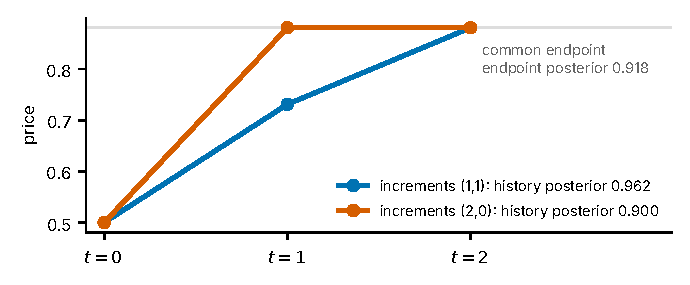
\includegraphics[width=0.72\linewidth]{generated/scale_example.pdf}
\caption{Two price paths from $p_0=1/2$ with the same endpoint under the unknown-scale model ($\Sigma_0=I_2$, $\boldsymbol a=(1,1)^{\mathsf T}$, $\alpha=\beta=1$, $\pi_0=1/2$). The endpoint posterior is $0.918$ for both. The history posteriors differ because residual variation is evidence about the noise scale.}
\label{fig:scale}
\end{figure} The distinction concerns probabilities and not necessarily decisions. For $\pi_0=1/2$ the history decision follows the sign of $U$, which in the aligned case agrees almost surely with the endpoint decision. The two classifiers then have equal error probability, yet deterministic integration gives Brier risks $0.108802$ (history) and $0.113789$ (endpoint), and log risks $0.357294$ and $0.378121$ nats. If $\alpha_n\to\infty$ with $\beta_n=\alpha_n/\lambda_0$, the log Bayes factors converge to the known-scale values $2\lambda_0U$ and $2\lambda_0Ms/C$, and the aligned gains vanish.

The direction of the effect gives a testable prediction.

\begin{corollary}[Residual variation shrinks endpoint evidence]
\label{cor:shrink}
Under \eqref{eq:scale-model} with $\boldsymbol a=(M/C)\Sigma_0\boldsymbol1\neq0$, let $E=R-S^2/C$, $U=MS/C$, $D=\beta+(E+S^2/C+J)/2$ and $\kappa=\alpha+T/2$. Then $\log\mathrm{BF}_{\rm H}=\kappa\log\{(D+U)/(D-U)\}$ and, for fixed $S$,
\[
 \frac{\partial\log\mathrm{BF}_{\rm H}}{\partial E}=-\frac{\kappa U}{D^2-U^2}.
\]
Since $D\pm U=\beta+(Z\pm\boldsymbol a)^{\mathsf T}K(Z\pm\boldsymbol a)/2\geq\beta>0$, the evidence $|\log\mathrm{BF}_{\rm H}|$ decreases in $E$ and tends to zero as $E\to\infty$.
\end{corollary}
\begin{proof}
Substitute $R=E+S^2/C$ and $U=MS/C$ in \eqref{eq:scale-bf} and differentiate, using $\partial D/\partial E=1/2$.
\end{proof}
To first order, $\log\mathrm{BF}_{\rm H}\approx2\kappa U/D$, which is $S$ times a decreasing function of $E$. A forecast that adds residual variation additively, as a squared-increment feature does, moves the log-odds the same way whatever the sign of $S$ and cannot express this shrinkage. Section~\ref{sec:confidence} tests the interaction directly.

\subsection{Mixtures of latent trading regimes}
\label{sec:mixture}
Let $K$ regimes have densities $g_k$, scales $s_k(v;\theta)>0$, outcome-dependent locations $m_{k,y}(v;\theta)$ and gates $\rho_k(v;\theta)$ with $\sum_k\rho_k=1$. Define
\begin{equation}
 f_y(z\mid v,\theta)=\sum_{k=1}^K\rho_k(v;\theta)\frac1{s_k(v;\theta)}g_k\!\left(\frac{z-m_{k,y}(v;\theta)}{s_k(v;\theta)}\right).
 \label{eq:mixture}
\end{equation}
A regime with $m_{k,1}>m_{k,0}$ responds positively to the outcome, and one with equal locations is outcome-independent. Regime names describe shapes of the increment law and carry no claim about trader identity.

\begin{assumption}[Product likelihood]
\label{ass:product}
Given $(Y,\theta)$ and the fixed design, the increments are independent with strictly positive densities \eqref{eq:mixture}, so $L_{y,T}(\theta;z,v)=\prod_{t=1}^Tf_y(z_t\mid v_t,\theta)$.
\end{assumption}
Let $\Pi$ be a proper nuisance prior independent of $Y$. The marginal likelihoods are $m_{y,T}=\int L_{y,T}\,\Pi(d\theta)$, the posterior is $\pi_T=\sigmoid(\logit\pi_0+\log\{m_{1,T}/m_{0,T}\})$, and the Jacobian from prices to increments cancels from the Bayes factor. Independence holds only given $\theta$. After integration the increments are dependent.

\begin{proposition}[Endpoint diagnostic]
\label{prop:mixture-endpoint-gradient}
Let $m_0,m_1$ be strictly positive $C^1$ densities on $\R^T$, $0<\pi_0<1$ and $\ell=\log(m_1/m_0)$. Then $S$ is sufficient for $Y$ if and only if
\begin{equation}
 \partial_{z_r}\ell(z)=\partial_{z_t}\ell(z)\quad\text{for all }z\in\R^T\text{ and all }r,t.
 \label{eq:mixture-gradient-test}
\end{equation}
Equivalently $\ell(z)=b(\boldsymbol1^{\mathsf T}z)$ for a $C^1$ function $b$. If \eqref{eq:mixture-gradient-test} fails, the optimal full-history forecast strictly improves expected Brier and log loss over the optimal endpoint forecast under the same densities.
\end{proposition}
This is the differentiable form of classical likelihood-ratio sufficiency \cite{pitman1936sufficient}. For a finite catalogue $m_y(z)=\sum_j\varpi_j\prod_tf_{yjt}(z_t)$ with masses $\varpi_j$ common to both outcomes, Appendix~\ref{app:mixture-endpoint} gives the score of $m_y$ in terms of the posterior responsibility of the shared state and of the component at each increment, so the test can be evaluated numerically.

\begin{proposition}[Common-tail obstruction]
\label{prop:mixture-endpoint-tail}
Let $T\geq2$ and
\[
 m_y(z)=\sum_{j=1}^J\varpi_j\prod_{t=1}^T f_{yjt}(z_t),
\]
with positive smooth $f_{yjt}$ and masses $\varpi_j$ common to both outcomes. Suppose
\begin{equation}
 \lim_{x\to+\infty}\frac{f_{1jt}(x)}{f_{0jt}(x)}=\lim_{x\to-\infty}\frac{f_{1jt}(x)}{f_{0jt}(x)}=1\quad\text{for all }j,t.
 \label{eq:mixture-common-tail}
\end{equation}
Then $S$ is sufficient for $Y$ if and only if $m_1=m_0$. Every outcome-informative member of this family therefore has a strictly positive model-based value of history beyond the endpoint.
\end{proposition}
The proof fixes a sum $s$ and takes $z_R=(R,\ldots,R,s-(T-1)R)$. All increments enter their tails while the sum stays $s$, so the likelihood ratio tends to one. An endpoint-only ratio would then equal one for every $s$. A positive Student component with outcome-independent weight, scale and degrees of freedom supplies \eqref{eq:mixture-common-tail} when all other components are Gaussian, and a finite outcome-dependent location shift leaves the leading tail unchanged. The condition covers the nine-state synthetic catalogue and the twelve-state empirical catalogue of Sect.~\ref{sec:empirical}. In the empirical catalogue, a positive-amplitude state has distinct outcome means at every positive volume, so the fitted family loses information at the endpoint whenever $T\geq2$. This statement concerns the full-support probability model. It gives no lower bound on an attainable gain and says nothing about the true market law.

Strict insufficiency can coexist with a negligible gain. Take an aligned Gaussian model with equal variances, $Z_t\mid Y\sim N(s_Y0.1,0.5^2)$ and $T=10$, where the endpoint is sufficient (Prop.~\ref{prop:ext-sufficiency}). Mixing in a centered Student-$t_5$ component of weight $\varepsilon$ and matched variance satisfies \eqref{eq:mixture-common-tail}, so the endpoint becomes insufficient for every $0<\varepsilon<1$. With a numerically approximated oracle endpoint posterior (Appendix~\ref{app:synthetic}), the gain $I(Y;Z\mid S)$ is about $6\times10^{-6}$ nats at $\varepsilon=0.001$, $9.2\times10^{-5}$ (Monte Carlo standard error $0.7\times10^{-5}$) at $\varepsilon=0.01$ and $1.27\times10^{-3}$ ($0.03\times10^{-3}$) at $\varepsilon=0.1$, against $I(Y;Z)\approx0.17$ (Fig.~\ref{fig:oracle} in Appendix~\ref{app:synthetic}). The smallest value is driven by rare draws, and independent runs range from $5.9$ to $7.1\times10^{-6}$. Proposition~\ref{prop:mixture-endpoint-tail} is therefore a statement about model specification. A fitted mixture with Student tails requires history dependence whether or not the data contain usable path information.

\section{Synthetic check}
\label{sec:synthetic}
We verify the calculations on the synthetic mixture of Appendix~\ref{app:synthetic}, with nine nuisance states and exact finite-prior integration. At $T=200$ with $\SimulationHistories$ test histories, finite-prior Bayes reaches Brier loss \PriorMarginalBrier{} and log loss \PriorMarginalLogLoss{}, against \PriorOracleBrier{} and \PriorOracleLogLoss{} when the generating state is known (Fig.~\ref{fig:scores} in Appendix~\ref{app:synthetic}). An intercept-and-slope recalibration of the endpoint logit, fitted on separate histories, is far worse: the full-history posterior minus the calibrated endpoint is \EndpointBrierDifference{} in Brier loss (95\% interval $[\EndpointBrierLower,\EndpointBrierUpper]$).

That gap mixes the intrinsic value of history with the calibrator's error. To separate them we fix the design at $v_t\equiv1$, the mean volume, and approximate the oracle endpoint posterior $r^*$ by convolving the one-step densities of each nuisance state on a grid. Halving the grid spacing and widening the support by half changes $r^*$ by at most $5\times10^{-8}$, so Monte Carlo error dominates. With $40{,}000$ prior-predictive histories per horizon, the intrinsic Brier gain $\E(q^*-r^*)^2$ is $0.0018$, $0.0039$, $0.0106$ and $0.0203$ at $T=5$, $10$, $25$ and $50$ (Monte Carlo standard errors at most $0.00012$), and the log gain $I(Y;Z\mid S)$ is $0.0036$, $0.0080$, $0.0223$ and $0.0450$ nats. The fitted calibrator's own error $\E(\widehat r-r^*)^2$ stays near $0.0009$ (Fig.~\ref{fig:oracle}). In this model the gap is mostly intrinsic, as Proposition~\ref{prop:mixture-endpoint-tail} allows but does not quantify. The generator uses the same volume relationship and tail law as the fitted model, so this is a specification check and says nothing about real markets.


\section{Evidence from Kalshi}
\label{sec:empirical}
\subsection{Cohort, timing and protocol}
We collected resolved binary BTC and ETH 15-minute contracts from Kalshi's public API, using transaction-close prices and traded quantities from one-minute candles \cite{kalshi2026candles,kalshi2026markets}. The sampling rule selects contracts closing on an exact UTC hour from 3 August to 27 September 2026. It selects 2,650 of 2,688 nominal slots, and the 38 absent slots fall in Thursday morning hours in both series. Every selected contract has a finalized binary outcome. Candle volumes sum exactly to the recorded lifetime volume for all 2,650 contracts, and a paginated trade check of one opening minute reconciles 1,643 executions with the candle. These checks establish consistency of the downloaded records and not independent verification of the exchange data.

Forecasts are issued five minutes (primary) and one minute (secondary) before scheduled close, and each uses only candles ending at least 60 seconds earlier. For a contract closing at 10:00, the 09:55 forecast uses candles ending no later than 09:54 and the 09:59 forecast uses candles ending no later than 09:58, so the final-minute settlement average never enters. The initial price $p_0$ is the close of the first candle, which ends one minute after the contract opens. A path therefore has 9 prices and 8 increments at the five-minute lead, and 13 prices and 12 increments at the one-minute lead. A record is excluded if any retained candle is missing, duplicated or untraded. No record was excluded. The reconstruction is retrospective, and the buffer is an assumption about publication latency.

We split by UTC close date into training (3--30 August, 1,322 contracts), validation (31 August--13 September, 664) and test (14--27 September, 664). Both assets and all intraday contracts of a date stay together, and every label used in fitting settled before the next period's first forecast. The protocol, written before collection, froze the models, the metrics and the bootstrap. The code writes predictions and a checksum lock before a separate stage opens test labels. This is a local safeguard and not an external preregistration. Appendix~\ref{app:empirical} gives the full specification, and an anonymized artifact contains the code, data, frozen models and predictions.\footnote{Anonymized artifact: \url{https://osf.io/ANONYMIZED}.}

\subsection{Forecasts and information sets}
\begin{table}[t]
\caption{Forecasts, their inputs and fitting windows. $x_t=\logit p_t$, $z_t=x_t-x_{t-1}$, $B$ is a log Bayes factor and ``asset'' an indicator. Ridge penalties for $P_{\rm lin}$, $H_{\rm log}$ and $E_{\rm log}$ are chosen from $\{0.01,0.1,1,10\}$ by validation log loss. $^\dagger$Added after test scores were seen.}
\label{tab:infosets}
\centering\scriptsize
\begin{tabular}{@{}llp{0.42\linewidth}l@{}}
\toprule
Name & Forecast & Inputs & Fitted on \\
\midrule
$P_{\rm last}$ & Latest price & $p_T$ & none \\
$P_{\rm lin}$ & Linear price calibration & $x_T$, asset & training \\
$P_{\rm cub}$ & Cubic price calibration & $x_T,x_T^2,x_T^3$, each also times asset & validation \\
$M$, $M_0$ & Mixture, with and without volume & $z_{1:T}$, $v_{1:T}$; training outcome rate & training \\
$P_{\rm cub}{+}M$ & Price plus mixture & $P_{\rm cub}$ inputs and $B_M(z,v)$ & validation \\
$G$ & Joint Gaussian history & $z_{1:T}$, asset & training \\
$P_{\rm cub}{+}G$ & Price plus Gaussian & $P_{\rm cub}$ inputs and $B_G(z)$ & validation \\
$H_{\rm log}$ & History logistic & $x_0$, $x_T$, last three increments summed, $\sum z_t^2$, volume-weighted mean increment, mean log volume, log-volume slope, asset & training \\
$E_{\rm log}^\dagger$ & Matched endpoint logistic & $H_{\rm log}$ inputs without the three path features & training \\
\bottomrule
\end{tabular}
\end{table}
Table~\ref{tab:infosets} lists every forecast. The mixture $M$ has two directional Gaussian components and a centered Student-$t_5$ component, with twelve nuisance states (three directional weights times four signal amplitudes) shared over each path and catalogue masses fitted by supervised EM. It combines the exact path likelihood ratio with the smoothed training outcome rate. Increments are invariant to the price level, so $M$ ignores $p_0$ and $p_T$: paths with identical increments starting at $0.1$ and $0.9$ get the same forecast. $M$ is an increment model with a common prior, and its standalone result evaluates a model subject to that restriction.

The incremental comparisons assess the empirical forecasting question. $P_{\rm cub}{+}M$ adds the single feature $B_M$ to $P_{\rm cub}$, with the same window, basis and penalty, so $P_{\rm cub}$ is its matched control. The combination enters $B_M$ as a regression feature with its own coefficient, which avoids counting overlapping evidence twice as adding it to the price log-odds would. $P_{\rm cub}$ is more flexible than $P_{\rm lin}$ but scores worse here, so it is a control and not the best price benchmark. The pair $H_{\rm log}$ and $E_{\rm log}$ is the comparison closest to the theory: both condition on $x_0$, $x_T$ and volume summaries, and differ by three path features. Volume summaries do not reproduce conditioning on the full design.

\subsection{Held-out results}

\begin{figure}[t]
\centering
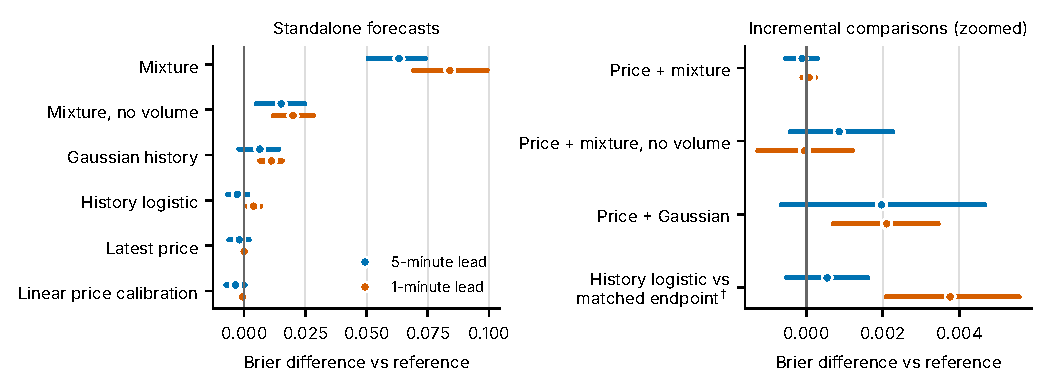
\includegraphics[width=\linewidth]{generated/empirical_differences_v2.pdf}
\caption{Paired held-out Brier differences. Left: standalone forecasts minus $P_{\rm cub}$. Right, on a finer scale: each combination minus $P_{\rm cub}$, and $H_{\rm log}$ minus $E_{\rm log}$ ($^\dagger$exploratory). Points are means and lines 95\% percentile intervals from 5,000 bootstrap resamples of whole UTC dates. Positive values favor the reference.}
\label{fig:differences}
\end{figure}
Fig.~\ref{fig:differences} and Table~\ref{tab:empirical-scores} in Appendix~\ref{app:empirical} give the results. Every difference below names its reference.

\paragraph{Incremental value.} Against $P_{\rm cub}$, adding the mixture signal changes Brier loss by $-0.00011$ ($[-0.00053,+0.00028]$) at five minutes and $+0.00008$ ($[-0.00011,+0.00024]$) at one minute. Leaving out one test date at a time moves the five-minute mean within $[-0.00019,+0.00001]$ and the one-minute mean within $[+0.00004,+0.00015]$, and the combination wins on 6 and 4 of the 14 dates (Fig.~\ref{fig:dates}, Appendix~\ref{app:empirical}). Adding the Gaussian signal costs $+0.0020$ ($[-0.0007,+0.0047]$) and $+0.0021$ ($[+0.0007,+0.0034]$). In the exploratory theory-matched pair (Brier $0.12633$ against $0.12578$ at five minutes, $0.06941$ against $0.06566$ at one minute), $H_{\rm log}$ minus $E_{\rm log}$ is $+0.0005$ ($[-0.0005,+0.0016]$) and $+0.0038$ ($[+0.0021,+0.0056]$): the path features did not help at five minutes and hurt at one minute. $E_{\rm log}$ was fitted after the test scores were seen. It is a pre-specified contrast for the later cohort of Sect.~\ref{sec:confidence}.

\paragraph{Standalone forecasts.} Against $P_{\rm lin}$, the mixture loses $+0.0668$ (interval $[+0.0566,+0.0754]$) at five minutes, with Brier losses $0.1923$ and $0.1255$. At one minute they are $0.1495$ and $0.0649$. By Proposition~\ref{prop:decomposition}, with $\mathcal E=\sigma(x_T,\text{asset})$ and $\mathcal H$ all observed path data, $\E(\widehat q-q^*)^2\ge R_B(\widehat q)-R_B(P_{\rm lin})$ for any history forecast, so the observed excess loss of $0.0668$ estimates a population lower bound on the mixture's mean squared distance from the best forecast based on all observed path data. On the validation window, the mixture's mean forecast ranges only from $0.45$ to $0.53$ across initial-price bins whose outcome rates range from $0.33$ to $0.71$ (Table~\ref{tab:validation-bins}). Within the central bin it still scores $0.196$ against $0.133$ for $P_{\rm lin}$ at five minutes. The pattern is consistent with the omitted price level contributing to the failure, but a binned comparison does not isolate that contribution. Removing volume improves the mixture to $0.1442$ and $0.0855$, still behind $P_{\rm lin}$. The ablation changes every volume-dependent gate, mean and variance at once, so it shows only that this volume specification hurts. $H_{\rm log}$ loses $+0.0008$ to $P_{\rm lin}$ at five minutes and $+0.0045$ at one minute.



\paragraph{Scope.} Intervals are descriptive and unadjusted for multiple comparisons. There are 14 date-level resampling units, the bootstrap ignores dependence across dates, and it treats the fitted forecasts as fixed. An interval containing zero is not evidence that the incremental information is zero. The cohort is one platform, two related crypto series and short paths of 8 or 12 increments, far shorter than the synthetic $T=200$. We make no claim about executable prices or trading returns.

\subsection{A test of the confidence mechanism}
\label{sec:confidence}
The comparisons above ask whether fitted history models add anything. Corollary~\ref{cor:shrink} names a specific way they could: residual variation should shrink the evidence in the endpoint. We test that mechanism with one feature. Let $S=x_T-x_0$, $E_\perp=\sum_t(z_t-S/T)^2$ (the residual energy with $\Sigma_0=I$) and
\[
 \phi=S\log(1+E_\perp/c),
\]
with $c$ the training median of $E_\perp$. The endpoint model $\widehat r$ is a penalized logistic regression on $b=(x_0$, the asset-specific cubic in $x_T$ of $P_{\rm cub}$, $\log(1+v_k)$ for every retained candle$)$. The history model $\widehat q$ adds $\phi$ with an unconstrained coefficient. Both are fitted on the training window with the penalty chosen on validation, as for $P_{\rm lin}$. The corollary predicts a negative coefficient. The training fits give $-0.0455$ at five minutes and $+0.514$ at one minute.

We froze both models and wrote the analysis plan before evaluating them on any test data. The gain is $G_B=R_B(\widehat r)-R_B(\widehat q)$, so positive values favor the history feature. The primary contrast is $G_B$ at five minutes, with log loss secondary and the one-minute lead as robustness. The smallest worthwhile gain is $\delta=0.001$, about $0.8\%$ of the five-minute baseline loss and twice the validation gain from recalibrating the raw last price. An interval entirely above $\delta$ reads as an improvement exceeding $\delta$, one inside $(-\delta,\delta)$ as practical equivalence, and one with upper bound below $\delta$ as excluding gains of $\delta$ or more. Intervals resample whole dates, with circular three-date blocks as a sensitivity fixed in advance.

\paragraph{Can the test detect the mechanism?} We ran the frozen procedure, with its features, penalty rule and decision rule, on data from the unknown-scale model with $T=8$, $\Sigma_0=I$, $\boldsymbol a=0.16\cdot\boldsymbol1$ and $\lambda\sim\operatorname{Gamma}(\alpha,\alpha/\lambda_0)$, $\lambda_0=1/0.49^2$, which matches the empirical increment scale and a five-minute Brier loss near $0.13$. Smaller $\alpha$ means more uncertainty about the noise scale and a larger oracle gain. In the \emph{naive} construction the price moves by the raw signal, $x_t=\sum_{j\le t}z_j$, and history informs reliability. In the \emph{efficient} construction the price is the public Bayesian posterior, $x_t=\log\mathrm{BF}_{\rm H}(z_{1:t})$, and history cannot help. Each of 200 replications per setting uses 1,322 training and 664 validation contracts and a test set of 664 contracts on 14 dates (the original test) or 2,350 on 49 dates (the later cohort). Table~\ref{tab:power} gives the results. Under efficient prices the fitted gain is centered at zero and the procedure manufactures no improvement, although its intervals exclude zero in $4$--$8\%$ of replications, above the nominal $2.5\%$. The date bootstrap is therefore somewhat liberal. With naive prices the fitted coefficient is negative in at least $96\%$ of replications for $\alpha\le8$, and the procedure recovers between about half and nearly all of the oracle gain. At the later-cohort size it detects a gain of $0.0044$ in $82\%$ of replications and a gain equal to $\delta$ in half. The efficient simulator checks the statistics only. Its price is a Bayesian posterior by construction and is not derived from traders' incentives.

\begin{table}[t]
\caption{Behavior of the frozen confidence test on simulated unknown-scale data, 200 replications per setting. Oracle gain is $\E(q^*-r^*)^2$. Achieved gain is the mean test $G_B$ with 664 test contracts. The last two columns give the frequency of an interval above zero and of an upper bound below $\delta=0.001$, with 664 and 2,350 test contracts.}
\label{tab:power}
\centering\scriptsize
\begin{tabular}{@{}lrrcc@{}}
\toprule
Setting & Oracle gain & Achieved gain & $\Prob(\text{lo}>0)$ & $\Prob(\text{hi}<\delta)$ \\
&&& 664 / 2{,}350 & 664 / 2{,}350 \\
\midrule
Efficient, $\alpha=1$ & $0.0000$ & $-0.00006$ & 0.04 / 0.04 & 0.63 / 0.86 \\
Efficient, $\alpha=3$ & $0.0000$ & $-0.00004$ & 0.07 / 0.08 & 0.61 / 0.82 \\
Efficient, $\alpha=8$ & $0.0000$ & $+0.00007$ & 0.06 / 0.06 & 0.61 / 0.82 \\
\addlinespace
Naive, $\alpha=1$ & $0.0135$ & $+0.00652$ & 0.60 / 0.98 & 0.00 / 0.00 \\
Naive, $\alpha=3$ & $0.0044$ & $+0.00340$ & 0.52 / 0.82 & 0.00 / 0.00 \\
Naive, $\alpha=8$ & $0.0010$ & $+0.00093$ & 0.29 / 0.50 & 0.14 / 0.12 \\
Naive, $\alpha=16$ & $0.0003$ & $+0.00017$ & 0.12 / 0.21 & 0.57 / 0.78 \\
\bottomrule
\end{tabular}

\end{table}

\paragraph{Original test window (exploratory).} This window had been used for the comparisons above. At five minutes $G_B=+0.00003$ ($[-0.00008,+0.00016]$), practical equivalence within $\delta$. At one minute $G_B=-0.00089$ ($[-0.00262,+0.00066]$), which excludes gains of $\delta$ or more. Both matched models score worse than $P_{\rm lin}$ (Brier $0.1264$ against $0.1255$ at five minutes).

\paragraph{Later cohort (confirmatory).} The cohort has 2,370 contracts on 50 UTC dates, closing from 01:00 UTC on 28 September to 16 November 2026. Two contracts closing at 00:00 UTC on 28 September were excluded in advance because their outcomes had been downloaded with the original listing. The 28 absent nominal slots are again Thursday-morning hours, candle volumes match lifetime volume for every contract, and no record was excluded. Models, protocol and file hashes were fixed before collection. Table~\ref{tab:confirm} gives the pre-specified contrasts.

At five minutes $G_B=+0.00008$ ($[-0.000001,+0.00016]$), positive on 27 of 50 dates and under every leave-one-date-out deletion. By the pre-declared rule this is practical equivalence within $\delta$. Under the three-date block sensitivity the lower bound is $+0.000001$, an improvement by the rule, but the gain is still a twelfth of $\delta$. The log-loss gain is $+0.00028$ ($[-0.000004,+0.00057]$). At one minute $G_B=+0.00003$ ($[-0.00066,+0.00071]$), also practical equivalence. Both matched models remain behind $P_{\rm lin}$ (Brier $0.1367$ against $0.1356$ at five minutes). Residual variation therefore shrinks the endpoint evidence in the predicted direction, but by too little to matter: a test that detects a gain of $\delta$ in half of simulated runs at this size bounds the gain below $0.00017$.

The frozen replication agrees with the original window. The mixture loses to $P_{\rm lin}$, the mixture signal adds nothing reliable to $P_{\rm cub}$, and the three path features of $H_{\rm log}$ again hurt at one minute. The raw last price beat $P_{\rm lin}$ by $0.0007$ ($[-0.0020,+0.0005]$) at five minutes, a sign that calibration drifts between periods.

\begin{table}[t]
\caption{Later cohort (2,370 contracts, 50 dates), pre-specified Brier contrasts with 95\% date-bootstrap intervals. The first row is a gain (positive favors the history feature). The others are differences (positive favors the reference).}
\label{tab:confirm}
\centering\scriptsize
\begin{tabular}{@{}lll@{}}
\toprule
Contrast & Five minutes & One minute \\
\midrule
Confidence test, $G_B$ & $+0.00008$ $[-0.000001,+0.00016]$ & $+0.00003$ $[-0.00066,+0.00071]$ \\
$P_{\rm cub}{+}M$ minus $P_{\rm cub}$ & $+0.00019$ $[-0.00001,+0.00039]$ & $-0.00005$ $[-0.00022,+0.00013]$ \\
$P_{\rm cub}{+}G$ minus $P_{\rm cub}$ & $-0.00003$ $[-0.00127,+0.00125]$ & $-0.00020$ $[-0.00118,+0.00075]$ \\
$H_{\rm log}$ minus $E_{\rm log}$ & $+0.00031$ $[-0.00011,+0.00073]$ & $+0.00222$ $[+0.00105,+0.00347]$ \\
$M$ minus $P_{\rm lin}$ & $+0.0533$ $[+0.0453,+0.0611]$ & $+0.0806$ $[+0.0727,+0.0885]$ \\
\bottomrule
\end{tabular}
\end{table}

\section{Discussion}
\label{sec:discussion}
Whether the endpoint keeps all outcome information depends on which nuisance quantities are unknown. An unknown amplitude preserves the alignment criterion, and an unknown common scale does not, because residual variation then tells how much to trust the endpoint. The common-tail result is a property of the fitted model and can carry a negligible gain.

Proposition~\ref{prop:decomposition} explains why the theory and the experiment can disagree, and Corollary~\ref{cor:shrink} gives the theory a direction to test. On Kalshi, fitted history signals added nothing reliable to matched price calibrations, in line with the martingale benchmark and with out-of-sample evidence from betting markets \cite{richard2021efficiency}. The confidence test makes this sharper. On an untouched cohort, a procedure that recovers most of a gain of $\delta$ in simulation found the predicted sign at five minutes and bounded the gain below a fifth of $\delta$. The mechanism is present in direction and negligible in size. For market design, $I(Y;\text{endpoint})$ and $I(Y;\text{history})$ should be reported together, since their difference can grow because the price aggregates worse.

We give no equilibrium foundation. Deriving the likelihood from traders with private signals, budgets and inventory, and bounding the mixture's approximation error, remain open. The theory conditions on the design and assumes independent increments given the shared nuisance. The cohort is one platform and two related series.

\bibliographystyle{splncs04}
\bibliography{references}

\appendix
\section{Gaussian endpoint sufficiency and score gains}
\label{app:gaussian-extension}
\paragraph{Proof of Proposition~\ref{prop:ext-sufficiency}.}
\begin{proof}
Expanding the Gaussian density makes its parameter-dependent factor
$\exp\{s_Y A U-A^2J_{\rm H}/2\}$. Integrating over $A$ gives the first
posterior formula and shows that $U$ is sufficient for $Y$.
Likewise $S\mid Y,A\sim N(s_Y AM,C)$, giving the second formula.

The identity
\[
 \Delta=
 \left(\boldsymbol a-\frac MC\Sigma\boldsymbol1\right)^\mathsf T
 \Sigma^{-1}
 \left(\boldsymbol a-\frac MC\Sigma\boldsymbol1\right)
\]
proves nonnegativity and its equality condition. If $\Delta=0$, then
$U=(M/C)S$, so the posteriors agree. This also covers
$\boldsymbol a=0$, when both equal $\pi_0$.

For the converse, suppose $\Delta>0$ and define
$R=U-(M/C)S$. Conditional on $(Y,A)$, $R$ and $S$ are independent and
\begin{equation}
 R\mid Y,A\sim N(s_Y A\Delta,\Delta).
 \label{eq:ext-residual}
\end{equation}
Indeed, $\operatorname{Cov}(U,S\mid Y,A)=M$ and
$\operatorname{Var}(U\mid Y,A)=J_{\rm H}$. Thus, conditional on every finite
$S=s$, the distribution of $U$ has a strictly positive density on $\R$.
For $j>0$, differentiation under the integral is justified by Gaussian
damping in $\alpha$, and
\[
 \frac{d}{du}\log\frac{G_j(u)}{G_j(-u)}
 =\frac{G'_j(u)}{G_j(u)}+\frac{G'_j(-u)}{G_j(-u)}>0.
\]
Strictness follows from $\nu((0,\infty))>0$. Consequently $q_{\rm H}$ is not
constant conditional on $S$, and cannot agree almost surely with $q_{\rm E}$.
The proper-score differences are
\begin{align*}
 \E[\mathcal L_{\log}(q_{\rm E},Y)-\mathcal L_{\log}(q_{\rm H},Y)]
 &=\E\KL\!\left(\operatorname{Bern}(q_{\rm H})\,
       \middle\|\,\operatorname{Bern}(q_{\rm E})\right),\\
 \E[(Y-q_{\rm E})^2-(Y-q_{\rm H})^2]
 &=\E[(q_{\rm H}-q_{\rm E})^2].
\end{align*}
Both are therefore strictly positive. Since fixed $p_0$ makes $p_T$ an
invertible transformation of $S$, the same conclusion holds for the terminal
price.
\end{proof}
\paragraph{Conditional information--MMSE identity.}
To verify \eqref{eq:ext-conditional-immse}, use the Markov relation
$Y\mathbin{-}X\mathbin{-}W_\gamma$ to write
$I(Y;W_\gamma)=I(X;W_\gamma)-I(X;W_\gamma\mid Y)$.
Apply the information--MMSE identity to both terms. Their derivative is
\[
 \frac12\left\{\E\operatorname{Var}(X\mid W_\gamma)
       -\E\operatorname{Var}(X\mid W_\gamma,Y)\right\}
 =\frac12\E\operatorname{Var}\!\left(\E[X\mid W_\gamma,Y]\mid W_\gamma\right).
\]
The last conditional variance has the binary expression in
\eqref{eq:ext-conditional-immse}; it is bounded in expectation by
$\E X^2=\E A^2$. Finite second moments justify the integrated identity.


\section{Endpoint insufficiency with an unknown common precision}
\label{app:scale-extension}

\paragraph{Proof of Proposition~\ref{prop:scale-sufficiency}.}
\begin{proof}
Let $Q_y(z)=(z-s_y\boldsymbol a)^\mathsf T K(z-s_y\boldsymbol a)$ and
$\kappa=\alpha+T/2$. Integrating the normal likelihood against the Gamma
density gives
\begin{equation}
 m_y(z)=\frac{\beta^\alpha\Gamma(\kappa)}
 {\Gamma(\alpha)(2\pi)^{T/2}|\Sigma_0|^{1/2}}
 \{\beta+Q_y(z)/2\}^{-\kappa}.
 \label{eq:scale-density}
\end{equation}
This is a multivariate Student density with $2\alpha$ degrees of freedom,
location $s_y\boldsymbol a$, and scale matrix $(\beta/\alpha)\Sigma_0$.
The scale matrix is not its covariance: the latter exists only for
$\alpha>1$ and equals $\beta\Sigma_0/(\alpha-1)$.
Since $Q_y=R+J-2s_yU$, taking the ratio proves the first formula in
\eqref{eq:scale-bf}. Applying the same integral to
$S\mid Y,\lambda\sim N(s_YM,C/\lambda)$ proves the second.

Write $b(z)=\beta+(R+J)/2$. Since $Q_0,Q_1\geq0$ and $\beta>0$,
$b(z)>|U(z)|$ and
\[
 \log\mathrm{BF}_{\rm H}(z)
 =2\kappa\operatorname{arctanh}\{U(z)/b(z)\}.
\]
If $T=1$, $S$ determines $Z$. If $\boldsymbol a=0$, both Bayes factors
are one. These cases give sufficiency.

Conversely let $T\geq2$ and $\boldsymbol a\ne0$. On the hyperplane
$\boldsymbol1^\mathsf Tz=s$, choose
$z_s=(s/C)\Sigma_0\boldsymbol1$ and any nonzero
$w\in\{w:\boldsymbol1^\mathsf Tw=0\}$. Then
\[
 R(z_s+tw)=s^2/C+t^2w^\mathsf TKw,\qquad
 U(z_s+tw)=Ms/C+t\boldsymbol a^\mathsf TKw.
\]
If $\boldsymbol a$ is not proportional to $\Sigma_0\boldsymbol1$, a
$w$ exists with $\boldsymbol a^\mathsf TKw\ne0$. Along this line
$U/b$ is not identically zero but tends to zero as $|t|\to\infty$.
Consequently the Bayes factor is nonconstant on every endpoint hyperplane.
If $\boldsymbol a=(M/C)\Sigma_0\boldsymbol1\ne0$, then $M\ne0$.
For every $s\ne0$, the numerator $U=Ms/C$ is nonzero and constant on the
hyperplane, while $b(z_s+tw)$ varies with $t$. Hence the Bayes factor is
again nonconstant there.

Both predictive densities are continuous and strictly positive on $\R^T$.
In linear coordinates $(S,W)$, their conditional densities for $W$ given
$S=s$ are therefore strictly positive on the whole $(T-1)$-dimensional
fiber. A continuous nonconstant Bayes factor takes different values on
nonempty relatively open subsets of that fiber. In the aligned case the
single exceptional value $s=0$ has probability zero. It follows that the
history posterior $q_{\rm H}$ is not measurable with respect to $S$.
Since $q_{\rm E}=\E[q_{\rm H}\mid S]$, the gains are
\begin{align*}
 G_B&=\E[(q_{\rm H}-q_{\rm E})^2]>0,\\
 G_{\log}&=\E\KL\{\operatorname{Bern}(q_{\rm H})
                  \|\operatorname{Bern}(q_{\rm E})\}>0.
\end{align*}
Expected Bayes Brier loss is at most $1/4$ and expected Bayes logarithmic
loss is at most $\log2$. Thus no finite observation moment is needed.
Fixed $p_0$ makes the endpoint an invertible transformation of $S$.
\end{proof}

\paragraph{Sufficiency before and after integration.}
For the original family indexed by $(y,\lambda)$, the likelihood ratio at
two sample points is
\[
 \frac{f_{y,\lambda}(z)}{f_{y,\lambda}(z')}
 =\exp\left[-\frac\lambda2
    \{R(z)-R(z')-2s_y(U(z)-U(z'))\}\right].
\]
It is independent of both parameters if and only if $R(z)=R(z')$ and
$U(z)=U(z')$. Thus $(U,R)$ is minimal sufficient for that family.
For the two marginalized distributions $m_0,m_1$, the usual likelihood-ratio
criterion instead makes $m_1/m_0$ itself minimal sufficient. The convenient
pair $(U,R)$ should not be called minimal for this binary experiment.

\paragraph{Residual energy and the decision boundary.}
In the aligned case, whiten the observation by $\Sigma_0^{-1/2}$ and
project onto the unit vector
$d=\Sigma_0^{1/2}\boldsymbol1/\sqrt C$. The projection is $S/\sqrt C$
and its squared orthogonal residual is $E=R-S^2/C$. The whitened mean is
parallel to $d$. Conditional on $(Y,\lambda)$, the residual is therefore
a centered $(T-1)$-dimensional normal vector with covariance
$I_{T-1}/\lambda$, independent of the projection. Its distribution does
not depend on $Y$, which also gives independence of $S$ and $E$ conditional
on $\lambda$. The chi-squared density yields
\eqref{eq:scale-residual-precision}. Since $\lambda$ is independent of $Y$,
$E$ is marginally independent of $Y$, although it is not independent of
$Y$ conditional on $S$.

More generally, holding $U$ fixed gives
\[
 \frac{\partial\log\mathrm{BF}_{\rm H}}{\partial R}
 =-\frac{\kappa U}{b^2-U^2}.
\]
Increasing residual energy therefore moves the posterior toward its prior
value in the aligned case. Since $b>|U|$, the sign of the history log
Bayes factor is the sign of $U$. The sign of the endpoint log Bayes factor
is the sign of $MS$. Equal priors and alignment consequently give identical
Bayes classifications except on a probability-zero tie set. This conclusion
does not extend in general to unequal outcome priors.

\paragraph{Known-scale limit, including expected losses.}
Take $\beta_n=\alpha_n/\lambda_0$ and $\alpha_n\to\infty$. For any fixed
$q\geq0$,
\[
 (\alpha_n+T/2)\log\{1+\lambda_0q/(2\alpha_n)\}
 \longrightarrow\lambda_0q/2.
\]
Applying this to $Q_0$ and $Q_1$ proves convergence of both Bayes factors
to the stated Gaussian formulas. The gamma-ratio asymptotic
$\Gamma(\alpha_n+T/2)/\{\Gamma(\alpha_n)\alpha_n^{T/2}\}\to1$
also shows that each density in \eqref{eq:scale-density} converges pointwise
to its $N(s_y\boldsymbol a,\Sigma_0/\lambda_0)$ density. Because all are
probability densities, Scheff\'e's lemma gives convergence in $L^1$.
The same argument applies to the endpoint densities.

For either experiment, write $m_n=\pi_0m_{1,n}+(1-\pi_0)m_{0,n}$ and
$q_n=\pi_0m_{1,n}/m_n$. The limits have positive densities, so $q_n\to q$
pointwise. Bayes Brier and log risks are respectively
$\int m_n q_n(1-q_n)$ and $\int m_n h(q_n)$, with
$h(q)=-q\log q-(1-q)\log(1-q)$. The integrands' posterior factors are
bounded continuous functions. Splitting each difference into a density
difference bounded by $\|m_n-m\|_1$ times its uniform bound, and a
posterior difference integrated against $m$, proves risk convergence by
dominated convergence. In the aligned Gaussian limit the gains are zero,
despite being strictly positive at every finite $\alpha_n$.

\section{Endpoint sufficiency for the finite mixture}
\label{app:mixture-endpoint}

\subsection{Pointwise and almost-sure formulations}
Fix $0<\pi_0<1$. Positivity gives a continuous posterior
$q(z)=\sigmoid(\logit\pi_0+\ell(z))$. Thus statistical sufficiency of
$S=\boldsymbol 1^{\mathsf T}Z$ is equivalent to
$\ell(z)=b(S)$ almost everywhere for some measurable $b$. The mixture density
$(1-\pi_0)m_0+\pi_0m_1$ is everywhere positive, so its null sets and Lebesgue
null sets agree.

Here the almost-everywhere qualifier can be removed. Use linear coordinates
$(s,u)\in\R\times\R^{T-1}$ with
$z=(u_1,\ldots,u_{T-1},s-\sum_{i<T}u_i)$, and write the transformed continuous
function as $F(s,u)$. Fubini's theorem implies that, for almost every $s$,
$F(s,u)=b(s)$ for almost every $u$. Continuity in $u$ extends this equality to
every $u$ for each such $s$. In particular,
$F(s,u)=F(s,0)$ on those fibers. Their $s$-values form a dense set, so continuity
in $s$ implies $F(s,u)=F(s,0)$ for every $(s,u)$. Hence
$\widetilde b(s)=F(s,0)$ supplies a $C^1$ pointwise version.

If $\ell(z)=\widetilde b(\sum_tz_t)$, the chain rule gives
\eqref{eq:mixture-gradient-test}. Conversely, that equation makes
$\nabla\ell(z)$ proportional to $\boldsymbol 1$. For any $z,z'$ on the same
sum hyperplane, the segment between them remains on that hyperplane and
\[
 \ell(z')-\ell(z)
 =\int_0^1\nabla\ell(z+u(z'-z))^{\mathsf T}(z'-z)\,du=0.
\]
All sum hyperplanes are connected. This proves
Proposition~\ref{prop:mixture-endpoint-gradient}, including the equivalence to
statistical sufficiency rather than merely a pointwise algebraic condition.
On a restricted support, connectedness of the relevant fibers must be
checked; the common-tail proposition additionally needs the stated full
unbounded support.

\subsection{Why the score improvement is strict}
Let $q_{\rm H}=\Prob(Y=1\mid Z)$ and
$q_{\rm E}=\Prob(Y=1\mid S)=\E(q_{\rm H}\mid S)$. Failure of the gradient
condition implies, by the preceding equivalence, that $q_{\rm H}$ is not
$S$-measurable up to a null set. Therefore
\[
 \E[(q_{\rm H}-q_{\rm E})^2]>0.
\]
Conditional expectation gives the Brier-risk difference exactly as this
quantity. Likewise, the logarithmic-risk difference equals
\[
 \E\!\left[
 D_{\rm KL}\{\operatorname{Bern}(q_{\rm H})
           \Vert\operatorname{Bern}(q_{\rm E})\}\right]
 = I(Y;Z\mid S)>0.
\]
Both optimal logarithmic risks are conditional entropies and are finite,
bounded by $H(Y)\leq\log2$. These are strict population comparisons between
optimal forecasts under one specified model. They are not guarantees for a
fitted classifier under an unknown data-generating distribution.

One can also see why a same-endpoint counterexample is not only a null-set
observation. Two unequal continuous values on one fiber persist in disjoint
neighborhoods and in nearby fibers. Positive densities assign positive
conditional mass to those fiber neighborhoods for almost every nearby sum.
The posterior then has positive conditional variance on a set of sums with
positive probability. The Fubini argument above formalizes this extension.

\subsection{The two levels of mixture responsibility}
All sums are finite, so differentiation commutes with summation without a
domination condition. Since the gates depend on the fixed design and not on
$z_t$,
\[
 \partial_{z_t}\log f_{yjt}(z_t)
 =\sum_k\frac{\rho_{jkt}g_{yjkt}(z_t)}{f_{yjt}(z_t)}
          \partial_{z_t}\log g_{yjkt}(z_t).
\]
Write $\tau_{yj}(z)=\varpi_j\prod_t f_{yjt}(z_t)/m_y(z)$ and
$\eta_{yjkt}(z_t)=\rho_{jkt}g_{yjkt}(z_t)/f_{yjt}(z_t)$.
Differentiate the product within each shared-state likelihood and then the
outer state mixture to obtain
\begin{equation}
 \partial_{z_t}\log m_y(z)
 =\sum_j\tau_{yj}(z)\sum_k\eta_{yjkt}(z_t)
       \partial_{z_t}\log g_{yjkt}(z_t).
 \label{eq:mixture-score-responsibilities}
\end{equation}
This is the elementary conditional-score identity of incomplete-data
likelihood calculations \cite{louis1982observed}, differentiated with respect
to an observation coordinate. The Gaussian component score is
$-(z_t-\mu)/\sigma^2$. For a Student component with location $\mu$, scale $b$,
and degrees of freedom $\nu$, the score is
\[
 -\frac{(\nu+1)(z_t-\mu)}{\nu b^2+(z_t-\mu)^2}.
\]
The checker evaluates both responsibility levels explicitly and compares the
resulting derivative with central differences of the production marginal
likelihood at fixed, unfitted parameter values.

\subsection{Independent-increment specialization}
\begin{proposition}[Common exponential tilt]
\label{prop:mixture-independent-tilt}
Let $T\geq2$ and suppose
$m_y(z)=\prod_t f_{yt}(z_t)$, where every $f_{yt}$ is a strictly positive $C^1$
density on $\R$. Then $\sum_tZ_t$ is sufficient for $Y$ if and only if there
exists one constant $c$ such that, for every $t$,
\begin{equation}
 f_{1t}(x)=\exp\{cx-\psi_t(c)\}f_{0t}(x),\qquad
 \psi_t(c)=\log\int_{\R}e^{cu}f_{0t}(u)\,du<\infty.
 \label{eq:mixture-common-tilt}
\end{equation}
The slope $c$ is common to all increments; the normalizing intercepts may
differ.
\end{proposition}
\begin{proof}
Write $h_t(x)=\log\{f_{1t}(x)/f_{0t}(x)\}$. The log Bayes factor is
$\sum_t h_t(z_t)$. By Proposition~\ref{prop:mixture-endpoint-gradient},
$h'_r(x)=h'_t(u)$ for all $x,u$ and any distinct $r,t$. Because $T\geq2$ and
the support is all of $\R^T$, one may vary either coordinate while holding the
other fixed. Every derivative must therefore be the same constant $c$.
Integration gives $h_t(x)=cx+b_t$; normalization of $f_{1t}$ implies
$b_t=-\psi_t(c)$ and finiteness of the integral. Conversely,
\eqref{eq:mixture-common-tilt} gives
$\ell(z)=c\sum_tz_t-\sum_t\psi_t(c)$, a function of the endpoint.
\end{proof}

If every one-step likelihood ratio tends to one at both tails, then
$cx+b_t\to0$ forces $c=0$ and $b_t=0$. Consequently endpoint sufficiency in
that independent-increment family requires identical outcome densities at
every step. This argument concerns a fixed sample dimension and a binary
experiment; it does not invoke an unrestricted fixed-dimensional-sufficiency
characterization for an entire parametric family.

\subsection{Proof of the common-tail proposition}
For any fixed $s\in\R$ and $R>0$, let
\[
 z_R=(R,\ldots,R,s-(T-1)R).
\]
Every coordinate tends to one of the two tails as $R\to\infty$, whereas its
sum remains $s$. For each catalogue state,
\[
 A_j(R)=\prod_{t=1}^T\frac{f_{1jt}(z_{R,t})}{f_{0jt}(z_{R,t})}\longrightarrow1.
\]
Writing the marginal likelihood ratio as a convex combination yields
\[
 \frac{m_1(z_R)}{m_0(z_R)}
 =\sum_j\frac{\varpi_j\prod_t f_{0jt}(z_{R,t})}{m_0(z_R)}A_j(R),\qquad
 \min_j A_j(R)\leq\frac{m_1(z_R)}{m_0(z_R)}\leq\max_j A_j(R).
\]
The finite catalogue makes both bounds tend to one. If $S$ were sufficient,
the pointwise version proved above would make this ratio equal to
$\exp\{b(s)\}$ for every $R$, hence $b(s)=0$. Since $s$ was arbitrary,
$m_1=m_0$. The converse is immediate. The strict-score statement follows from
the earlier risk identities.

The proof requires common outcome-specific catalogue masses. It does not
justify an exchange of a tail limit and an arbitrary continuous nuisance
integral. Nor does it apply unchanged after censoring, truncation, or clipping
has replaced the full-support observation law.

For a Student component with a fixed finite location, positive scale $b$, and
degrees of freedom $\nu$, its density has leading term
$c_\nu b^\nu |x|^{-(\nu+1)}$ at either tail. If its mixing weight, scale, and
$\nu$ do not depend on the outcome, that term is identical for both outcomes;
finite Gaussian components decay faster. This proves
\eqref{eq:mixture-common-tail} for the stated empirical and synthetic
catalogues, including the shifted Student component in the latter.

Finally, the empirical mean calculation does not assume a favorable fitted
weight vector. Its Student component is centered, so at normalized volume
$r>0$ the sign of the directional mean for $a>0$ is the sign of
\[
 w(1+r)^{1/2}-\frac{1-w}{4}(1+r)^{3/10}
 =(1+r)^{3/10}\left[w(1+r)^{1/5}-\frac{1-w}{4}\right].
\]
For $w\geq1/5$, the bracket is strictly positive when $r>0$. The catalogue
contains positive amplitudes and its smoothed masses are positive, giving
opposite nonzero marginal means under the two outcomes at any such time.
The outcome laws are therefore distinct. If all volumes are zero, all
location shifts vanish and this informativeness argument does not apply.

\section{Synthetic model and outcome identification}
\label{app:synthetic}
\subsection{The synthetic experiment}
Write $s_y=2y-1$ and $a(v)=\operatorname{expit}((v-1.5)/0.3)$. The simulations use
\begin{align}
 Z\mid k=1,y,v,\theta&\sim N\!\left(s_y\mu(1-e^{-0.1v}),\frac{0.3^2}{1+0.05v}\right),\nonumber\\
 Z\mid k=2,y,v,\theta&\sim N(0,0.5^2),\label{eq:example}\\
 Z\mid k=3,y,v,\theta&\sim -s_y\,0.3a(v)+0.4\,t_5,\nonumber
\end{align}
where $0.4$ is the scale of the Student distribution. The gate has exponents $(0.5,0,0.3)$:
\[
 \rho_k(v;\theta)=\frac{\omega_k(1+v)^{\gamma_k}}{\sum_j\omega_j(1+v)^{\gamma_j}},\qquad
 (\omega_1,\omega_2,\omega_3)=\left(w,\tfrac{2(1-w)}3,\tfrac{1-w}3\right).
\]
The nuisance parameter is $\theta=(w,\mu)$. Volumes are i.i.d.\ Gamma$(2,0.5)$ and $p_0=\pi_0=1/2$. Each scenario uses 2,000 test histories, balanced across outcomes, at horizons $T\in\{10,25,50,100,200,500\}$. The fixed-default scenario sets $(w,\mu)=(0.4,0.5)$. The prior-predictive scenario draws one state per history from the uniform prior on $\{0.15,0.4,0.65\}\times\{0.25,0.5,0.75\}$. Marginal likelihoods sum the nine full-path likelihoods in log space, which is exact integration for a discrete prior. The calibrated endpoint is an intercept and slope on the terminal logit, fitted on a separate set of 2,000 training histories per scenario and horizon. The two ablations replace volume by $1$ or the Student component by a variance-matched Gaussian.

\subsection{Outcome identification}
Let $P_{y,\theta}^{(T)}$ be the product law of Assumption~\ref{ass:product}. At truth $(y^*,\theta^*)$ define
\begin{equation}
 \delta_T=\inf_{\theta\in\Theta}\frac1T\KL\!\left(P_{y^*,\theta^*}^{(T)}\,\middle\|\,P_{1-y^*,\theta}^{(T)}\right).
 \label{eq:gap}
\end{equation}
The same nuisance value must explain the whole path. Outcome identification differs from endpoint sufficiency: a full history may separate outcomes while its endpoint discards information.

\begin{proposition}[Orientation symmetry]
\label{prop:symmetry}
Suppose $\Psi:\Theta\to\Theta$ is a measurable involution and $f_1(\cdot\mid v,\theta)=f_0(\cdot\mid v,\Psi\theta)$ on the design. Then $\delta_T=0$ at every truth. If also $\Pi\circ\Psi^{-1}=\Pi$, then $m_{1,T}=m_{0,T}$ for every path and $\pi_T=\pi_0$ for every $T$.
\end{proposition}
\begin{proof}
The opposite outcome with parameter $\Psi\theta^*$ reproduces the true law. Changing variables by $\Psi$ in the marginal likelihood and using prior invariance proves the second assertion.
\end{proof}
An unknown common orientation multiplying both directional means in \eqref{eq:example}, with equal prior mass on $+1$ and $-1$, gives this symmetry. Restricting the orientation removes it and is a substantive prior restriction.

\begin{proposition}[A checkable separation condition]
\label{prop:sign}
Let $I_T\subset\{1,\ldots,T\}$. Suppose that for each $t\in I_T$ there is a measurable set $A_t$ and a constant $d>0$, uniform in $T$, such that
\[
 P_{y^*,\theta^*}(Z_t\in A_t)\geq b_t+d,\qquad
 \sup_{\theta\in\Theta}P_{1-y^*,\theta}(Z_t\in A_t)\leq b_t.
\]
Then $\delta_T\geq 2d^2|I_T|/T$.
\end{proposition}
\begin{proof}
The difference on $A_t$ bounds total variation below by $d$. Pinsker's inequality bounds each relevant KL divergence below by $2d^2$. Sum these bounds before taking the infimum in \eqref{eq:gap}.
\end{proof}

\subsection{Horizon scores and oracle endpoint posteriors}
\begin{figure}[h]
\centering
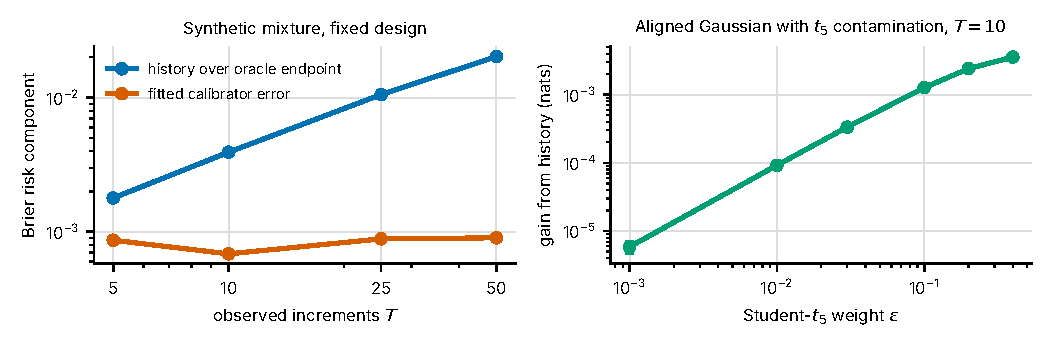
\includegraphics[width=\linewidth]{generated/oracle_endpoint.pdf}
\caption{Left: Brier components of Proposition~\ref{prop:decomposition} for the synthetic mixture at fixed design, comparing the exact history posterior with the numerically approximated oracle endpoint posterior (blue) and the error of a fitted intercept-and-slope endpoint calibrator (orange). Right: gain from history in an aligned Gaussian model with a centered Student-$t_5$ contamination of weight $\varepsilon$, with $\pm2$ Monte Carlo standard errors. The left panel uses $40{,}000$ histories per point. The right panel uses stratified sampling on the number of contaminated increments for $\varepsilon\le0.1$ and $400{,}000$ plain draws above.}
\label{fig:oracle}
\end{figure}
\begin{figure}[t]
\centering
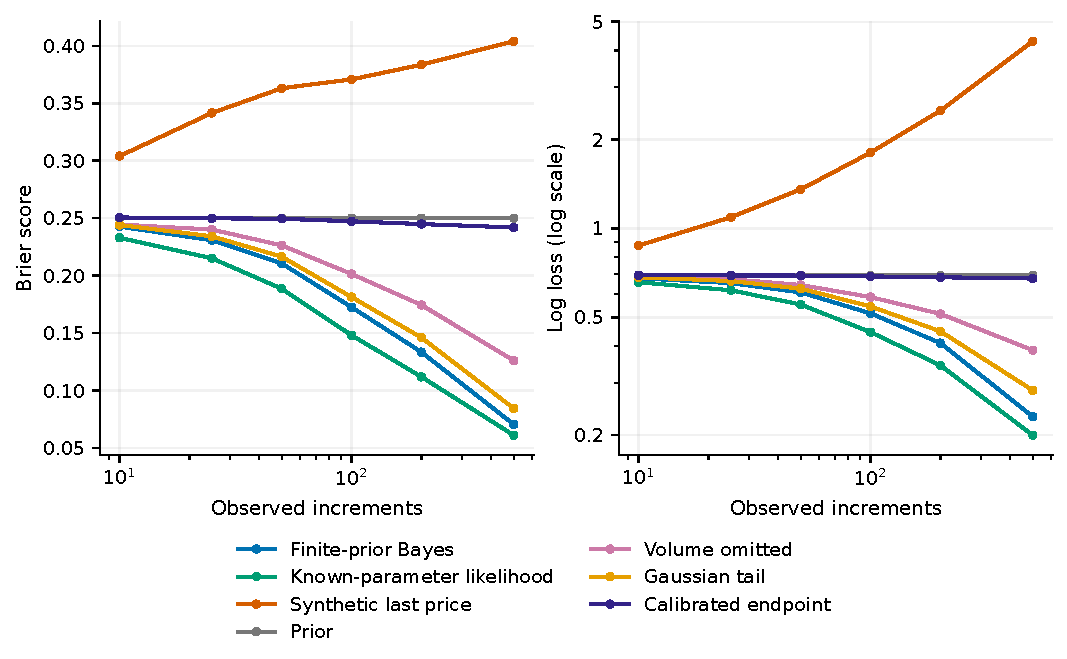
\includegraphics[width=\linewidth]{generated/revised_scores.pdf}
\caption{Synthetic proper scores against horizon under prior-predictive simulation. The calibrated endpoint uses independent training histories. Lines show sample means over 2,000 histories. The right panel has a logarithmic vertical axis.}
\label{fig:scores}
\end{figure}
For the oracle comparison of Sect.~\ref{sec:synthetic} the design is fixed at $v_t\equiv1$. For each outcome and nuisance state, the one-step density is evaluated on a grid of spacing $h=0.002$ over $[-L_T,L_T]$ with $L_T=0.15T+5\sqrt T+25$, normalized, and raised to the $T$-th power in the Fourier domain. The endpoint density is the uniform mixture of the nine convolved densities, and $r^*$ is obtained by linear interpolation of the two log densities at the observed sum. Repeating the computation with $h=0.001$ on $[-1.5L_T,1.5L_T]$ changes $r^*$ by at most $3.7\times10^{-8}$ on the simulated histories and the reported gains by less than $10^{-11}$. Monte Carlo standard errors of the intrinsic gains are at most $1.2\times10^{-4}$ (Brier) and $2.8\times10^{-4}$ nats (log). The endpoint calibrator is an unpenalized intercept-and-slope logistic regression on $S$, fitted on $2{,}000$ independent histories.

The contamination study uses the same convolution with a single state, $Z_t\mid Y\sim(1-\varepsilon)N(s_Y0.1,0.5^2)+\varepsilon\,0.5\sqrt{3/5}\,t_5$ and $T=10$, on $[-1.5L,1.5L]$ with $L=20+3\sqrt{10}$ and $h=0.001$, which agrees with the coarser grid to within $5\times10^{-8}$ in $r^*$. Plain Monte Carlo is unreliable at small $\varepsilon$ because the gain comes from rare large draws. For $\varepsilon\le0.1$ we therefore stratify on the number $K$ of contaminated increments, draw $10^5$ histories with $K=k$ for $k=0,\ldots,5$, and weight the stratum means by the Binomial$(10,\varepsilon)$ probabilities. The omitted mass $\Prob(K>5)$ is at most $1.5\times10^{-4}$. The resulting gains are $9.2\times10^{-5}$ ($\pm0.7\times10^{-5}$), $3.34\times10^{-4}$ ($\pm0.16\times10^{-4}$) and $1.27\times10^{-3}$ ($\pm0.03\times10^{-3}$) at $\varepsilon=0.01$, $0.03$ and $0.1$. At $\varepsilon=0.001$ three independent runs, with $10^5$ or $10^6$ draws per stratum, gave $5.9$, $6.3$ and $7.1\times10^{-6}$, a spread larger than their nominal standard errors, so we report only the order of magnitude. Above $\varepsilon=0.1$ we use $400{,}000$ plain draws.

\section{Empirical specification}
\label{app:empirical}
\subsection{Observations}
For a contract opening at $o$ and closing at $o+900$ seconds, the candle ending at $o+60k$ gives the transaction close $p_{k-1}$ and the traded quantity $v_{k-1}$, $k\geq1$. A forecast issued $\ell$ minutes before close uses candles ending at or before $o+900-60(\ell+1)$, giving prices $p_0,\ldots,p_T$ with $T=8$ for $\ell=5$ and $T=12$ for $\ell=1$. Increments are $z_t=\logit\bar p_t-\logit\bar p_{t-1}$ with $\bar p=\min\{\max\{p,\epsilon\},1-\epsilon\}$, and $z_t$ is paired with the volume $v_t$ of the candle that closes it. The primary clipping is $\epsilon=0.001$ and the sensitivity is $\epsilon=0.005$. Every model and comparator is fitted separately for each lead and clipping level, and by asset where stated.

\subsection{Mixture}
Pool the training increments and set $s=\max\{1.4826\operatorname{MAD}(z),0.05\}$. Let $m_v$ be the median positive training volume, $r=v/m_v$ and $g(r)=2r/(1+r)$. The catalogue is the Cartesian product $w\in\{0.2,0.5,0.8\}$, $a\in\{0,0.1,0.3,0.6\}$, twelve states shared by all increments of a path. With $q=2y-1$ and $\mu_j=a_js$, the gates are the normalized values of
\[
 \bigl(w_j(1+r)^{1/2},\ (1-w_j)(1+r)^{3/10}/2,\ (1-w_j)/2\bigr)
\]
and the components are
\[
 N\!\Bigl(q\mu_jg(r),\frac{s^2}{1+0.25r}\Bigr),\qquad N\!\bigl(-0.5q\mu_jg(r),s^2\bigr),\qquad t_5\bigl(0,s\sqrt{3/5}\bigr),
\]
with variances in the Gaussian arguments. The no-volume variant sets $r\equiv1$ in fitting and prediction. The catalogue masses $\pi$ maximize the training conditional likelihood $\sum_i\log\sum_j\pi_j\prod_tf_{y_i,j}(z_{it}\mid v_{it})$ plus $(1/12)\sum_j\log\pi_j$ by EM from $\pi_j=1/12$, stopping when the relative objective change is below $10^{-9}$ or after 2,000 iterations. The forecast is $\operatorname{expit}\{\logit p_Y+B_M\}$, where $B_M=\log\{\sum_j\pi_j\prod_tf_{1,j}\}-\log\{\sum_j\pi_j\prod_tf_{0,j}\}$ is the log Bayes factor, with $p_Y=(\sum_iy_i+0.5)/(n+1)$. All fits converged (388 and 191 iterations at the two leads with volume, 500 and 250 without). Fitted values at $\epsilon=0.001$ are $s=0.490$ and $0.603$ and $m_v=19{,}677$ and $24{,}088$ contracts. At the five-minute lead the masses concentrate on $(w,a)=(0.2,0)$, $(0.2,0.6)$ and $(0.5,0.6)$, with $0.28$, $0.23$ and $0.44$.

\subsection{Comparators}
Logistic models standardize features $u_i$ with the means and standard deviations of their fitting sample and minimize the summed objective
\[
 \sum_{i=1}^n\bigl[\log\{1+e^{\beta_0+\beta^{\mathsf T}u_i}\}-y_i(\beta_0+\beta^{\mathsf T}u_i)\bigr]+\frac\lambda2\|\beta\|_2^2
\]
by L-BFGS, with the intercept $\beta_0$ unpenalized. $P_{\rm lin}$, $H_{\rm log}$ and $E_{\rm log}$ are fitted on training data with the penalty from $\{0.01,0.1,1,10\}$ minimizing validation log loss. $P_{\rm cub}$ and the combinations are fitted on validation data with $\lambda=1$. The features of $P_{\rm cub}$ are $x_T,x_T^2,x_T^3$, the asset indicator, and its products with the three powers, so it has an asset-specific intercept and cubic. In the combinations, $B_M$ or $B_G$ is one further feature. In $H_{\rm log}$ the volume features use $\log(1+v_t)$ over all retained candles, the slope is its least-squares slope on centered time, and the volume-weighted increment is $\sum_tz_tv_t/\sum_tv_t$. The Gaussian history model fits, per asset, class means $m_0,m_1$ and the shared covariance $0.9S+0.1\operatorname{diag}(S)$ of within-class residuals, with diagonal floor $10^{-4}$, and uses $B_G=(z-(m_0+m_1)/2)^{\mathsf T}\Sigma^{-1}(m_1-m_0)$ with an asset-specific smoothed prior.

\subsection{Original-window scores}
\begin{table}[h]
\caption{Held-out losses on the same 664 contracts at each lead (14 UTC dates, 332 contracts per asset). Lower is better. Names follow Table~\ref{tab:infosets}.}
\label{tab:empirical-scores}
\centering\scriptsize
\begin{tabular}{lrrrr}
\toprule
 & \multicolumn{2}{c}{5-minute lead} & \multicolumn{2}{c}{1-minute lead} \\
Method & Brier & Log loss & Brier & Log loss \\
\midrule
Training frequency & 0.2506 & 0.6944 & 0.2506 & 0.6944 \\
Initial price & 0.2303 & 0.6520 & 0.2303 & 0.6520 \\
$P_{\rm last}$, latest price & 0.1271 & 0.3998 & 0.0655 & 0.2138 \\
$P_{\rm lin}$, linear price calibration & 0.1255 & 0.3941 & 0.0649 & 0.2120 \\
$P_{\rm cub}$, cubic price calibration & 0.1290 & 0.4042 & 0.0655 & 0.2117 \\
$H_{\rm log}$, history logistic & 0.1263 & 0.3968 & 0.0694 & 0.2232 \\
$M$, mixture & 0.1923 & 0.5660 & 0.1495 & 0.4695 \\
$M_0$, mixture without volume & 0.1442 & 0.4431 & 0.0855 & 0.2835 \\
$P_{\rm cub}{+}M$ & 0.1289 & 0.4041 & 0.0656 & 0.2119 \\
$P_{\rm cub}{+}M_0$ & 0.1299 & 0.4060 & 0.0655 & 0.2120 \\
$G$, joint Gaussian history & 0.1355 & 0.4168 & 0.0766 & 0.2500 \\
$P_{\rm cub}{+}G$ & 0.1310 & 0.4083 & 0.0676 & 0.2174 \\
$E_{\rm log}^\dagger$, matched endpoint logistic & 0.1258 & 0.3955 & 0.0657 & 0.2139 \\
\bottomrule
\end{tabular}

\end{table}

\subsection{Sensitivity and diagnostics}
At the five-minute lead no observed price lies outside $[0.005,0.995]$, so both clipping levels give identical results. At the one-minute lead, with $\epsilon=0.005$, the scores of Table~\ref{tab:empirical-scores} change by less than $0.001$ in Brier loss. The mixture minus $P_{\rm lin}$ is $+0.0848$ ($[+0.0697,+0.1002]$) and $P_{\rm cub}{+}M$ minus $P_{\rm cub}$ is $+0.00016$ ($[-0.00016,+0.00043]$). Table~\ref{tab:validation-bins} gives the validation diagnostic by initial price.

\begin{table}[h]
\caption{Validation window, five-minute lead: mean forecast and Brier loss of the mixture $M$ and of $P_{\rm lin}$ by initial-price bin.}
\label{tab:validation-bins}
\centering\scriptsize
\begin{tabular}{lrrrrrr}
\toprule
$p_0$ bin & $n$ & Outcome rate & Mean $M$ & Mean $P_{\rm lin}$ & Brier $M$ & Brier $P_{\rm lin}$ \\
\midrule
$<0.30$ & 14 & 0.357 & 0.457 & 0.288 & 0.220 & 0.133 \\
$[0.30,0.45)$ & 162 & 0.333 & 0.451 & 0.364 & 0.215 & 0.129 \\
$[0.45,0.55)$ & 258 & 0.484 & 0.486 & 0.504 & 0.196 & 0.133 \\
$[0.55,0.70)$ & 209 & 0.569 & 0.522 & 0.632 & 0.192 & 0.137 \\
$\geq0.70$ & 21 & 0.714 & 0.531 & 0.747 & 0.162 & 0.064 \\
\bottomrule
\end{tabular}

\end{table}

\begin{figure}[h]
\centering
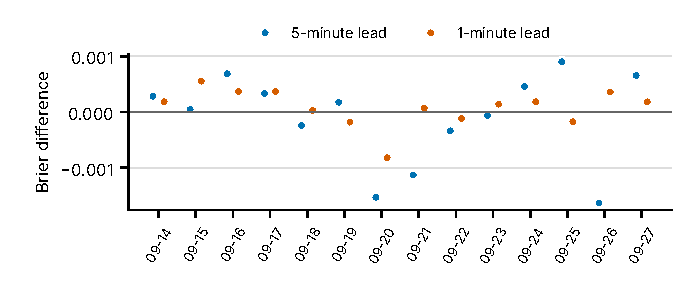
\includegraphics[width=0.72\linewidth]{generated/date_differences.pdf}
\caption{Date-level mean Brier difference, $P_{\rm cub}{+}M$ minus $P_{\rm cub}$, on the 14 test dates.}
\label{fig:dates}
\end{figure}

\subsection{Artifact}
The anonymized artifact contains the collection scripts with checksummed raw responses, the protocol and model-design documents written before collection, the evaluation and model code with tests, the frozen fitted models and prediction lock, the held-out predictions and scores, and the scripts for every figure and diagnostic in this paper.

\section{Supporting concentration and error bounds}
\label{app:supporting-rate}
\label{sec:concentration}
The following standard marginal-likelihood argument separates assumptions about likelihood behavior from assumptions about prior mass; see also \cite{chatterjee2020bayes} for general Bayes-factor convergence results. Fix an infinite deterministic design $(v_t)_{t\geq1}$ and the corresponding product probability law $P_*$ at $(y^*,\theta^*)$. Every almost-sure statement below refers to this one law. Write
\[
 \ell_{y,T}(\theta)=\log L_{y,T}(\theta),\quad
 \Lambda_{y,T}(\theta)=T^{-1}\E_*\ell_{y,T}(\theta),\quad
 a_{y,T}=\sup_{\theta\in\Theta}\Lambda_{y,T}(\theta).
\]
Assume these expectations and suprema are finite and the following sets and suprema are measurable.

\begin{assumption}[Uniform likelihood control and prior mass]
\label{ass:rate}
For both outcomes,
\[
 u_{y,T}:=\sup_\theta|T^{-1}\ell_{y,T}(\theta)-\Lambda_{y,T}(\theta)|\longrightarrow0
 \quad P_*\text{-almost surely}.
\]
For every $\epsilon>0$, the set
$A_{y,T}(\epsilon)=\{\theta:\Lambda_{y,T}(\theta)\geq a_{y,T}-\epsilon\}$ has positive prior mass and
\[
 -T^{-1}\log\Pi(A_{y,T}(\epsilon))\longrightarrow0.
\]
\end{assumption}
Positive mass for each finite $T$ is insufficient: a set whose mass decreases exponentially can change the leading marginal-likelihood rate. A fixed finite nuisance prior with all masses positive satisfies the second condition automatically when $\Theta$ equals its support. On such a support, a strong law for each log likelihood implies the first condition because only finitely many likelihoods need simultaneous control.

\begin{lemma}[Signed Bayes-factor rate]
\label{thm:rate}
Under Assumptions~\ref{ass:product} and \ref{ass:rate}, with $\theta^*\in\Theta$,
\begin{equation}
 \frac{s_{y^*}}{T}\log\BF_T=\delta_T+o(1)\qquad P_*\text{-almost surely}.
 \label{eq:rate}
\end{equation}
If $\liminf_T\delta_T>0$, then $\Prob(Y=y^*\mid Z_{1:T},v_{1:T})\to1$ almost surely and
\[
 -T^{-1}\log\Prob(Y\ne y^*\mid Z_{1:T},v_{1:T})=\delta_T+o(1).
\]
\end{lemma}
The proof in Appendix~\ref{app:rate} keeps the near-optimal prior mass explicitly. This is an almost-sure exponent for posterior error along paths. It is not automatically the exponent of the expected error or the optimal classification risk.

\subsection{A finite-prior bound without bounded increments}
\label{sec:finite}
Now let $\Pi=\sum_{j=1}^Jw_j\delta_{\theta_j}$ with $w_j>0$, and suppose the true nuisance value is $\theta_{j^*}$. Denote $w_*=w_{j^*}$ and prior outcome odds against the truth by $r=\Prob(Y=1-y^*)/\Prob(Y=y^*)$. For $s\in(0,1)$ define the fractional affinity
\begin{equation}
 A_{j,T}(s)=\prod_{t=1}^T\int_{\R}
 f_{y^*}(z\mid v_t,\theta_{j^*})^{1-s}
 f_{1-y^*}(z\mid v_t,\theta_j)^s\,dz.
 \label{eq:affinity}
\end{equation}
Each factor belongs to $(0,1]$ by H\"older's inequality. Gaussian and Student components do not require bounded log-likelihood ratios for this definition.

\begin{proposition}[Finite-prior posterior error]
\label{prop:finite}
Let $e_T=\Prob(Y\ne y^*\mid Z_{1:T},v_{1:T})$ and
$C_T(s)=(r/w_*)^s\sum_j w_j^s A_{j,T}(s)$. Under Assumption~\ref{ass:product},
\begin{align}
 \E_* e_T&\leq\min\{1,C_T(s)\},\label{eq:expected}\\
 P_*(e_T\geq\epsilon)&\leq\min\left\{1,\left(\frac{1-\epsilon}{\epsilon}\right)^s C_T(s)\right\},\quad 0<\epsilon<1.
 \label{eq:tail}
\end{align}
For equal nuisance weights and equal outcome priors,
\[
 \E_*e_T\leq\min\{1,J\exp[-Tc_T(s)]\},\qquad c_T(s)=\min_j[-T^{-1}\log A_{j,T}(s)].
\]
\end{proposition}
The proof uses a lower bound on the true marginal likelihood and fractional powers of a finite sum (Appendix~\ref{app:finite}). The factor $w_*^{-s}$ exposes the cost of a prior that gives the truth little mass. The bound may be uninformative at short horizons. It does not extend unchanged to a continuous prior or to truth outside the support, and the affinity rate is distinct from the KL rate in Lemma~\ref{thm:rate}.


\section{Supporting local stability bound}
\label{app:supporting-stability}
\label{sec:stability}
\subsection{Perturbing increments and volumes}
Fix $R,V<\infty$. Suppose, uniformly over $y,\theta$, the log densities satisfy
\begin{equation}
 |\log f_y(z\mid v,\theta)-\log f_y(z'\mid v',\theta)|
 \leq L_z|z-z'|+L_v|v-v'|
 \label{eq:lipschitz}
\end{equation}
for $z,z'\in[-R,R]$ and $v,v'\in[0,V]$. The prior and the initial conditioning information remain the same for the two records. For a finite nuisance catalogue of smooth positive component densities and smooth gates, such bounds hold on compact observation domains when scales stay positive. Merely bounding increments while leaving all volumes unbounded does not ensure a uniform Gaussian score bound in \eqref{eq:example}, because its first component's scale shrinks with volume.

\begin{proposition}[Local posterior stability]
\label{prop:stability}
For two records satisfying \eqref{eq:lipschitz}, set
$D=L_z\sum_t|z_t-z'_t|+L_v\sum_t|v_t-v'_t|$. Then
\begin{equation}
 |\log\BF_T(z,v)-\log\BF_T(z',v')|\leq2D,\qquad
 |\pi_T(z,v)-\pi_T(z',v')|\leq D/2.
 \label{eq:stability}
\end{equation}
\end{proposition}
The first inequality follows by integrating the pathwise likelihood bounds; the second uses $\sup_x\sigmoid'(x)=1/4$. Appendix~\ref{app:stability} supplies the details and the computable constants used in the experiments. The bound is local to both records, not just the unperturbed one.

Stability depends on the measurement scale. If all prices in both records lie in $[\varepsilon,1-\varepsilon]$, then
\[
 \sum_{t=1}^T|z_t-z'_t|
 \leq\frac{2}{\varepsilon(1-\varepsilon)}\sum_{t=0}^T|p_t-p'_t|.
\]
The constant diverges near the boundary. Log-odds modeling therefore requires more care with extreme prices, even though it removes support constraints for density modeling.


\section{Posterior belief change and information}
\label{app:belief-change}
\label{sec:information}
Define the realized posterior-to-prior divergence
\begin{equation}
 \IG(z,v)=\pi_T\log\frac{\pi_T}{\pi_0}+(1-\pi_T)\log\frac{1-\pi_T}{1-\pi_0}.
 \label{eq:ig}
\end{equation}
It is nonnegative and at most $\max\{-\log\pi_0,-\log(1-\pi_0)\}$, interpreting $0\log0=0$. For the symmetric prior its ceiling is $\log2$ nats. For an asymmetric prior, the general upper bound is attained at the endpoint with smaller prior mass. Writing $u=\log\BF_T$ and $q(u)=\sigmoid(\logit\pi_0+u)$ gives
\[
 \frac{d}{du}\KL(\operatorname{Bern}(q(u))\|\operatorname{Bern}(\pi_0))
 =u\,q(u)\{1-q(u)\}.
\]
The divergence increases away from zero along each branch. Only when $\pi_0=1/2$ is it a single function of $|u|$.

Under the full prior-predictive model for the fixed design, with $\theta\sim\Pi$ as well as $Y\sim\operatorname{Bern}(\pi_0)$,
\begin{equation}
 \E_{\mathrm{prior}}\IG(Z_{1:T},v_{1:T})
 = I(Y;Z_{1:T}\mid v_{1:T})\leq h(\pi_0),
 \label{eq:mi}
\end{equation}
where $h(q)=-q\log q-(1-q)\log(1-q)$. For nested designs the expected information cannot decrease; individual realized information paths can decrease after contradictory observations. Averaging at a fixed nuisance truth does not generally equal the mutual information of the nuisance-integrated model.

Equation~\eqref{eq:mi} holds under the assumed joint law. A misspecified likelihood can produce large $\IG$ while assigning high probability to wrong outcomes. We therefore report Brier loss $(q-y)^2$ and logarithmic loss $-y\log q-(1-y)\log(1-q)$ alongside information gain. Both are strictly proper \cite{gneiting2007strictly}, whereas information gain alone cannot reward accurate forecasts over confident mistakes.



\section{Bayes-factor rate and posterior concentration}
\label{app:rate}
Fix $\epsilon>0$ and one outcome $y$. The upper bound follows directly from the uniform likelihood deviation:
\[
 m_{y,T}\leq\exp\{T(a_{y,T}+u_{y,T})\}.
\]
Restricting the integral to $A_{y,T}(\epsilon)$ gives
\[
 m_{y,T}\geq\Pi(A_{y,T}(\epsilon))
 \exp\{T(a_{y,T}-\epsilon-u_{y,T})\}.
\]
Consequently,
\begin{equation}
 a_{y,T}-\epsilon-u_{y,T}+T^{-1}\log\Pi(A_{y,T}(\epsilon))
 \leq T^{-1}\log m_{y,T}\leq a_{y,T}+u_{y,T}.
 \label{eq:laplace-bounds}
\end{equation}
Take a probability-one set on which the likelihood deviations converge for both outcomes, apply the prior-mass assumption for a countable sequence $\epsilon\downarrow0$, and conclude
$T^{-1}\log m_{y,T}-a_{y,T}\to0$.

Under the true model, nonnegativity of KL gives
$a_{y^*,T}=\Lambda_{y^*,T}(\theta^*)$. Moreover,
\[
 a_{1-y^*,T}=\Lambda_{y^*,T}(\theta^*)-\delta_T.
\]
Subtracting the two log marginal likelihoods proves \eqref{eq:rate}. Let $c=\log\{\Prob(Y=y^*)/\Prob(Y=1-y^*)\}$ and
$b_T=\log\{m_{y^*,T}/m_{1-y^*,T}\}$. Then
\[
 e_T=(1+e^{c+b_T})^{-1},\qquad
 -T^{-1}\log e_T=T^{-1}\log(1+e^{c+b_T}).
\]
When $\liminf\delta_T>0$, we have $b_T/T=\delta_T+o(1)$ and $c+b_T\to\infty$, proving both consistency and the posterior error exponent.

For the finite nuisance catalogue in the simulations with iid exogenous volumes, apply a strong law to the joint observations $(Z_t,V_t)$ for each of the finitely many outcome--parameter pairs. Absolute log-density expectations are finite in the stated model: the positive Student component supplies a polynomial lower tail, volumes have Gamma tails, and the data have finite second moments. For each pair $(y,j)$, also apply the strong law to $h_{y,j}(V_t)=\E_*[\log f_y(Z_t\mid V_t,\theta_j)\mid V_t]$. This function is integrable by the preceding absolute-integrability argument. Subtracting the two strong laws gives
\[
 \frac1T\sum_{t=1}^T\{\log f_y(Z_t\mid V_t,\theta_j)-h_{y,j}(V_t)\}\to0.
\]
Taking a finite maximum verifies the conditional-design likelihood deviations for almost every realized volume design, by disintegration of the joint probability-one event. Candidate-wise KL averages also converge, yielding a volume-averaged minimum over the finite support. This argument does not establish the result for every possible deterministic design.

\section{Finite-prior fractional-moment bound}
\label{app:finite}
Write $L_*=L_{y^*,T}(\theta_{j^*})$ and $L_j^-=L_{1-y^*,T}(\theta_j)$. Since $m_{y^*,T}\geq w_*L_*$, the posterior odds against the truth obey
\[
 O_T=\frac{\Prob(Y=1-y^*)m_{1-y^*,T}}{\Prob(Y=y^*)m_{y^*,T}}
 \leq R_T:=\frac r{w_*}\sum_{j=1}^Jw_j\frac{L_j^-}{L_*}.
\]
For $0<s<1$, $(\sum_j a_j)^s\leq\sum_j a_j^s$ for nonnegative $a_j$. Therefore
\[
 \E_*R_T^s\leq\left(\frac r{w_*}\right)^s
 \sum_jw_j^s\E_*\left(\frac{L_j^-}{L_*}\right)^s
 =C_T(s),
\]
where independence under the true law gives the product in \eqref{eq:affinity}. Because
$e_T=O_T/(1+O_T)\leq\min\{1,R_T\}\leq R_T^s$,
\eqref{eq:expected} follows. The event $e_T\geq\epsilon$ implies
$R_T\geq\epsilon/(1-\epsilon)$. Markov's inequality applied to $R_T^s$ proves \eqref{eq:tail}. For uniform weights and $r=1$, the factors $J^s$ and $J^{-s}$ cancel inside each term, leaving $\sum_j A_{j,T}(s)\leq J e^{-Tc_T(s)}$.

The proof does not treat a marginal Bayes factor as an independent-increment sum. It also avoids conditioning on a truncation event, which would change the expectations used to center a concentration inequality.

\section{Stability and computable score bounds}
\label{app:stability}
For each fixed $y,\theta$, summing \eqref{eq:lipschitz} gives
\[
 e^{-D}L_{y,T}(\theta;z',v')\leq L_{y,T}(\theta;z,v)
 \leq e^D L_{y,T}(\theta;z',v').
\]
Integrating against the same prior preserves these inequalities. Hence each log marginal likelihood changes by at most $D$, and the log Bayes factor changes by at most $2D$. Composing with the logistic function proves the posterior bound.

For a positive mixture with weights independent of $z$,
\[
 \partial_z\log f_y(z\mid v,\theta)
 =\sum_k r_k(z,v,y,\theta)\,\partial_z\log f_{k,y}(z\mid v,\theta),
\]
where $r_k=\rho_kf_{k,y}/f_y$ are nonnegative responsibilities summing to one. The absolute mixture score is therefore bounded by the largest absolute component score. On $|z|\leq R$, a Gaussian with mean $m$ and standard deviation $\sigma$ has score at most $(R+|m|)/\sigma^2$. For a Student component with location $m$, scale $s$, and $\nu$ degrees of freedom,
\[
 \left|\partial_z\log f(z)\right|
 =\frac{(\nu+1)|z-m|}{\nu s^2+(z-m)^2}
 \leq\frac{\nu+1}{2s\sqrt\nu}.
\]
Unlike a Gaussian log density, this Student log density has a globally bounded location score.

For unchanged volumes, set $R_t=\max\{|z_t|,|z'_t|\}$ at each time. Evaluate the component bounds using $R_t$ and $v_t$, then maximize across times, both outcomes, and all catalogue states. The resulting $L_z$ certifies
$|\log\BF_T-\log\BF'_T|\leq2L_z\sum_t|z_t-z'_t|$ for that pair of records. This is a pathwise bound using the actual perturbations. Replacing the sum by a noise standard deviation would not give a deterministic bound.

For price perturbations, the mean value theorem bounds each logit difference by
$|p_t-p'_t|/[\varepsilon(1-\varepsilon)]$. The triangle inequality for adjacent increments then gives the price-scale bound in the main text. Since the analysis fixes $p_0$, an increment distance is adequate; if initial states can vary, it is only a pseudometric on complete price histories unless the initial state is included.


\end{document}
